\documentclass[12pt]{article}
\usepackage[T1]{fontenc} 
\usepackage[portuguese]{babel}
\usepackage{hyphenat}
% use se você precisar forçar a separação de sílabas em quebra de linha
\hyphenation{mate-mática recu-perar}
\usepackage{graphicx}
\graphicspath{images/}
\usepackage{csquotes}
\usepackage{subfiles}
\usepackage{amsmath}
\usepackage{csvsimple} 
\usepackage{geometry}
\usepackage{tabularx} % tabelas com colunas espaçadas igualmente
\usepackage{booktabs} % linhas divisórias das tabelas
\usepackage{amsfonts} % mathbb
\usepackage[hidelinks]{hyperref} % referencas dentro do documento




% BEGIN RASCUNHO
% \usepackage{datetime2}
% \usepackage{fancyhdr}
% \pagestyle{fancy}
% \fancyhf{} % limpa tudo
% \fancyhead[L]{\scriptsize\textsf{VERSÃO PRELIMINAR}} % texto pequeno no canto esquerdo do rodapé
% \fancyhead[R]{\scriptsize\textsf{\DTMnow}} % texto pequeno no canto esquerdo do rodapé
% \renewcommand{\headrulewidth}{0pt} % remove linha do cabeçalho
% \renewcommand{\footrulewidth}{0pt} % remove linha do rodapé

% \usepackage{draftwatermark}
% \SetWatermarkText{\textsf{RASCUNHO}}
% \SetWatermarkScale{3}
% END RASCUNHO


\usepackage{tikz}
\usetikzlibrary{arrows.meta, positioning}

\geometry{
    a4paper,
    left=3cm,
    top=3cm,
    right=2cm,
    bottom=2cm
}
\setlength{\parindent}{4em}
%\setlength{\parskip}{1em}
\renewcommand{\baselinestretch}{1.5}

\usepackage[dvipsnames]{xcolor}
\definecolor{alert}{RGB}{201, 58, 128}
\setlength {\marginparwidth }{2cm} 
\usepackage[colorinlistoftodos]{todonotes}
\usepackage{comment}
\usepackage{subcaption}
\DeclareUnicodeCharacter{0301}{*************************************}
\usepackage{enumitem}
%% CSS: mudando o gerenciador de bibliografia para biblatex para contornar 
% alguns problemas. Adendo: a compilação no overleaf ficou muito instável 
% e por alguma razão não imprime a seção de bibliografia no final, apesar
% de colocar as anotações ao longo do texto. Voltando ao bibtex no momento (5/9/2024)
%\usepackage{biblatex}
%\addbibresource{ref.bib}

%% TODO:
% - Resolver a questão com biblatex no overleaf

% LZT (23/04/25) fiz alteração manual para and others no bib e parece ter resolvido. tambem mudei o estilo das referencias

\title{TÍTULO}
\author{autor}

\begin{document}

% CAPA
\thispagestyle{empty}
\begin{flushright}
    \begin{huge}
     \textbf{RELATÓRIO}\\[3,5cm]
    \end{huge}
    %% CSS: Podemos usar um título mais genérico agora e depois discutir um definitivo
    {\bf \LARGE  CLASSIFICAÇÃO DE GLAUCOMA EM IMAGENS DE FUNDO DE OLHO COM APRENDIZAGEM PROFUNDA}\\
    \bigskip 
    Leandro Zangirolami Trovões (Orientando)\\
    Carlos da Silva dos Santos (Orientador)\\
    Universidade Federal do ABC\\[5,5cm]
\end{flushright}
\vfill
\begin{center}
    Santo André,\\
    Abril de 2025
\end{center}
\newpage


% RESUMO
\begin{center}
\noindent{\bf \Large Resumo}
\end{center}

\begin{quote}
O glaucoma é a principal causa de cegueira irreversível no mundo, com projeção de atingir até 111,8 milhões de pessoas em 2040. Caracterizada pelo dano progressivo ao nervo óptico, a doença é assintomática em seus estágios iniciais, tornando o diagnóstico precoce essencial para seu controle. O exame de fundo de olho permite a identificação de sinais característicos da doença, e técnicas de aprendizagem profunda têm demonstrado grande potencial na triagem automatizada.

Este trabalho propôs o desenvolvimento de um sistema baseado em redes neurais convolucionais para a detecção de casos referenciáveis para avaliação de glaucoma em imagens de fundo de olho. O sistema é composto por três etapas principais: segmentação do disco óptico, classificação binária para glaucoma, e classificação multi-rótulo das características clínicas justificadoras, utilizando o conjunto de dados JustRAIGS.

No conjunto de teste definido, o modelo atingiu sensitividade de 89,72\% em 95\% de especificidade e AUC-ROC de 0,9781 na tarefa de classificação binária. Na tarefa de classificação multi-rótulo, obteve distância de Hamming de 0,12960. O sistema apresentou desempenho competitivo em relação a trabalhos recentes da literatura, demonstrando sua aplicabilidade como ferramenta auxiliar na triagem de glaucoma.
\end{quote}

\begin{center}
Santo André, abril de 2025
\end{center}

\newpage


\begin{center}
\noindent{\bf \Large Abstract}
\end{center}

\begin{quote}

Glaucoma is the leading cause of irreversible blindness worldwide, with projections estimating up to 111.8 million affected individuals by 2040. Characterized by progressive damage to the optic nerve, the disease is asymptomatic in its early stages, making early diagnosis crucial for its management. Fundus imaging enables the identification of characteristic signs of glaucoma, and deep learning techniques have shown great potential for automated screening.

This work proposes the development of a system based on convolutional neural networks for the detection of referable glaucoma cases in fundus images. The system comprises three main stages: optic disc segmentation, binary classification for glaucoma, and multi-label classification of clinical justifications, using the JustRAIGS dataset.

On the defined test set, the proposed model achieved a sensitivity of 89.72\% at 95\% specificity and an AUC-ROC of 0.9781 in the binary classification task. In the multi-label classification task, it achieved a Hamming distance of 0.12960. The system demonstrated competitive performance compared to recent works in the literature, supporting its applicability as an auxiliary tool for glaucoma screening.

\end{quote}

\begin{center}
Santo André, abril de 2025
\end{center}

\newpage

\tableofcontents

\newpage


\section{Introdução}
\label{sec:introducao}

Principal causa de cegueira irreversível no mundo \cite{steinmetz_causes_2021}, o glaucoma é uma doença sem cura, caracterizada pelo dano progressivo ao nervo óptico \cite{who_2019}. Estima-se que, em 2020, 3,6 milhões de pessoas com 50 anos ou mais já tenham perdido a visão para o Glaucoma \cite{steinmetz_causes_2021} e um estudo de 2014 ainda projeta que 111.8 milhões de pessoas sejam afetadas pela doença no ano de 2040 \cite{tham_global_2014}.

O estágio inicial do glaucoma é assintomático, mas a doença causa perda progressiva da visão periférica conforme avança e pode levar à perda total da visão. O tratamento pode retardar ou prevenir a progressão, mas depende de um diagnóstico precoce, geralmente antes mesmo dos primeiros sintomas \cite{who_2019}.

Uma das formas de identificar a presença de glaucoma é por meio da \emph{fundoscopia} ou exame de fundo de olho, no qual é possível observar alterações características, muitas vezes antes mesmo que a perda de visão se torne detectável \cite{weinreb_2004}. Um exemplo de imagem obtida nesse exame é apresentado na Figura~\ref{fig:fundus}.

% [LZT] TODO: investigar discordacias com o que é dito no JustRAIGS
% talvez falar: tradicionalmente usava-se o CDR, mas agora outras características são avaliadas...
A principal característica observada ao analisar o fundo de olho é o tamanho da \emph{escavação} em relação ao tamanho do disco óptico do paciente, ambos destacados na Figura~\ref{fig:disk}. O disco óptico é a região em que as células da retina se convergem para formar o nervo óptico. Essa convergência forma uma depressão ao centro do disco, chamada de escavação (em inglês conhecido como \emph{optic cup}). O \emph{anel neurorretiniano} é a região que envolve a escavação. A razão entre o tamanho do disco e da escavação é conhecida como razão disco-copo (em inglês \emph{cup-to-disk ratio}) e seu valor acima do normal é um indicativo do dano causado pela doença \cite{weinreb_2004}. % posso também citar weinreb_2016 para essa última afirmação

\begin{figure}[htb]
 \centering
 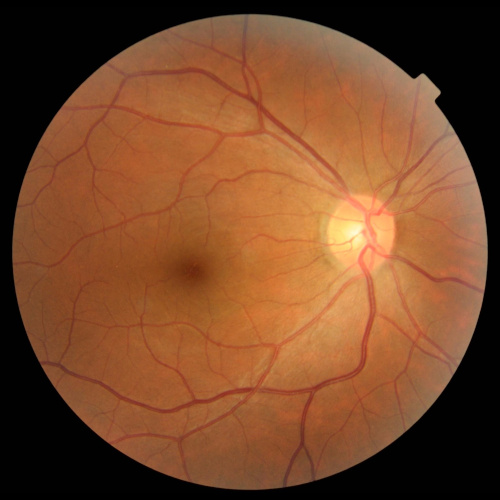
\includegraphics[width=0.3\textwidth]{images/TRAIN000004_cut.JPG}
 \caption{Imagem de fundo de olho. Obtida do banco de dados JustRAIGS~\cite{justraigs}.}
 \label{fig:fundus}
\end{figure}

% entretanto a análise manual por oftalmologistas é sujetivel a falhas

Com o avanço das técnicas de aprendizagem profunda, modelos de redes neurais convolucionais têm se mostrado promissores na análise automática de imagens de fundo de olho para auxílio no diagnóstico do glaucoma \cite{li_review_2021}, sendo capazes de até mesmo superar a avaliação humana~\cite{tan_glaucoma_2020}. No entanto, desafios persistem, como a escassez de grandes bases de dados anotadas e a necessidade de aumentar a interpretabilidade dos modelos~\cite{li_review_2021}.

\begin{figure}[htb]
 \centering
 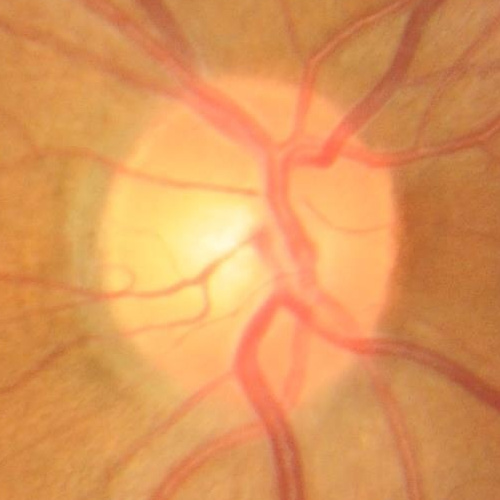
\includegraphics[width=0.3\textwidth]{images/disk.jpg}
 \caption{Disco óptico em destaque. Obtida do banco de dados JustRAIGS~\cite{justraigs}.}
 \label{fig:disk}
\end{figure}

Neste trabalho, exploramos o uso de aprendizagem profunda para a detecção de casos referenciáveis de glaucoma em imagens de fundo de olho. Para isso, utilizamos o banco de dados JustRAIGS~\cite{justraigs}, que além das classificações principais, inclui anotações adicionais que justificam a decisão clínica.

%% [CSS]: Incluir um parágrafo aqui para dizer:
% - o justRAIGS é ligado a uma competição; a competição é composta por duas fases. Na primeira, predizer se a imagem de fundo de olho é referenciada ou não para glaucom. Na segunda, predizer quais indicativos de diagnóstico estão presentes na imagem referenciada. 
% - na construção do nosso modelo, usamos a mesma estrutura da competição. Como a competição se encerrou e o conjunto de avaliação é fechado, não é possível determinar qual classificação  nosso modelo alcançaria. Mas adotamos uma avaliação com conjunto de teste independente que torna a comparação possível com os resultado publicados.
% - incluir aqui o resultado de sensibilidade obtido no conjunto de teste, comparar com os melhores resultados publicados.

% LZT: incluido, e removi a seguinte frase do paragrafo anteriro para evitar duplicação
% > Buscamos não apenas realizar a classificação binária, mas também desenvolver um classificador multi-rótulo que aponte as anotações adicionais definidas no JustRAIGS, de modo a fornecer justificativa para a decisão.

O conjunto JustRAIGS foi disponibilizado como parte da competição promovida pelo 21\textsuperscript{o} \textit{IEEE International Symposium on Biomedical Imaging} (ISBI 2024), intitulada \textit{Justified Referral in AI Glaucoma Screening --- JustRAIGS}. Ela é composta por duas tarefas principais: (i) predizer se a imagem de fundo de olho deve ser referenciada para avaliação de glaucoma e (ii) predizer quais indicativos de diagnóstico justificam a referência. O sistema desenvolvido neste trabalho adota a mesma estrutura proposta.

Como a competição já havia se encerrado no momento da realização deste trabalho e o conjunto de avaliação é fechado, não é possível determinar qual classificação nosso modelo alcançaria. Entretanto, empregamos um conjunto de teste independente, o que possibilita uma comparação aproximada com os resultados publicados. Nesse conjunto, nosso modelo obteve uma sensitividade de 89,72\% em 95\% de especificidade mínima na primeira tarefa e uma distância de Hamming de 0,12960 na segunda. Para referência, durante a competição, Zhang et al.~\cite{justraigs_zhang} alcançaram uma sensitividade de 87,00\% em 95\% de especificidade e distância de Hamming de 0,239, enquanto Kubrak~\cite{justraigs_kubrak} obteve 90,90\% de sensitividade e distância de Hamming de 0,1280.

O restante deste texto está organizado da seguinte maneira: a Seção~\ref{sec:objetivo} apresenta os objetivos do trabalho. A Seção~\ref{sec:review} discute conceitos fundamentais de aprendizagem profunda e visão computacional aplicados à tarefa, além de apresentar os bancos de dados utilizados e trabalhos relacionados. A metodologia proposta é detalhada na Seção~\ref{sec:methodology}, os resultados obtidos são discutidos na Seção~\ref{sec:results}, e as conclusões são apresentadas na Seção~\ref{sec:conclusions}.

\begin{comment}
DESCONSIDERAR ESSE BLOCO

usando redes neurais\\
e até mesmo técnicas de processamento de sinais\cite{Noronha2014}

porem:
\begin{itemize}
 \item datasets limitados (agora temos um de 100k imagens) e alguns são privados
 \item falta de justificativa, blackbox ~\cite{li_review_2021} 7.2.5, usar features adicionais para explicar decisão
\end{itemize}

suposições que precisam ser sustentadas:\\
1- razão OD e OC é a melhor forma de identificar glaucoma\\
2- CNN é melhor de que calcular a razão ente OD e OC: [Chen, 2015] afirma mas não sustenta. Cita [3]\\

2) Diaz-Pinto, 2019: usando CNN não precisa fazer segmentação perfeita do OD e do OC
"Important limitations of the methods that are based on handcrafted characteristics (CDR, Area Cup/Disc ratio (ACDR), vessel kinks and ISNT rule) is the significant disagreement in estimating them even between expert human graders. For that reason, new algorithms have been focused on automatic feature extraction such as the data-driven methods [3] and convolutional neural networks (CNNs)."\\
Menciona alguns trabalhos que foram pela abordagem da segmentação e os resultados obtidos.

investigar:
Chen, 2015: 17 5 6 14, 2, 12, 13\\
Noronha, 2014: 9, 16, 17, 18

\end{comment}


\bigskip

\section{Objetivos}
\label{sec:objetivo}

O objetivo geral deste trabalho é desenvolver e avaliar um sistema baseado em aprendizagem profunda para a identificação de casos referenciáveis de glaucoma em imagens de fundo de olho, 
%% CSS: alterando para minimizar a ênfase em interpretação, veja se concorda; redação original segue abaixo em comentário
% buscando também fornecer interpretações que justifiquem a decisão do modelo.
buscando também fornecer predições sobre características adicionais (p.ex. presença de hemorragia) que justifiquem a decisão do modelo.

Os objetivos específicos são:
\begin{itemize}
    \item Desenvolver um método de segmentação do disco óptico, delimitando a região de interesse (ROI) nas imagens de fundo de olho;
    \item Treinar um classificador binário para glaucoma;
    \item Treinar um classificador multi-rótulo para identificar características específicas associadas ao glaucoma, com base nas anotações adicionais do conjunto JustRAIGS;
    %% CSS: Avaliar o trabalho é o esperado; poderia haver um objetivo relacionado a isso se o trabalho criticasse os métodos de avaliação atuais/propusesse um arcabouço de avaliação próprio
    %\item Avaliar o desempenho dos modelos propostos utilizando métricas apropriadas de classificação e segmentação;
    \item Comparar os resultados obtidos com aqueles reportados na literatura recente, especialmente trabalhos utilizando o conjunto de dados JustRAIGS.
\end{itemize}

\bigskip

\section{Revisão Bibliográfica}
\label{sec:review}

Iniciamos esta seção com uma revisão dos fundamentos de aprendizagem profunda e redes neurais convolucionais. Em seguida, apresentamos algumas bases de dados públicas utilizadas na construção de sistemas automatizados para detecção de glaucoma, bem como trabalhos anteriores relacionados. Detalhamos o conjunto de dados JustRAIGS e a competição a ele atrelado, que serve de referência para este trabalho, e apresentamos alguns dos trabalhos submetidos. Por fim, descrevemos as principais métricas empregadas na avaliação de classificadores e segmentadores.

\subsection{Aprendizado de Máquina}
\label{sec:review:machine_learning}

O aprendizado de máquina é uma subárea da inteligência artificial, definida em 1959 por Arthur Samuel como o campo de estudo que dá aos computadores a habilidade de aprender sem serem explicitamente programados. Posteriormente, Tom Mitchell (1997) formalizou o conceito, definindo que um programa de computador \textbf{aprende} com a experiência $E$ em relação a uma classe de tarefas $T$ e uma medida de desempenho $P$, se seu desempenho nas tarefas de $T$, medido por $P$, melhora com a experiência $E$ \cite{mitchell1997machine}.

As tarefas de aprendizado de máquina podem ser classificadas em diferentes categorias, de acordo com o tipo de sinal de resposta (\textit{feedback}) disponível para o sistema \cite{russell2010artificial}:

\begin{itemize}
    \item \textbf{Aprendizado não supervisionado}: o algoritmo deve identificar padrões nos dados de entrada sem receber \emph{feedback} explícito. A tarefa mais comum nessa categoria é o agrupamento de dados (\textit{clustering});
    
    \item \textbf{Aprendizado supervisionado}: o algoritmo recebe pares de dados entrada-saída e deve aprender uma função que mapeie as entradas para as saídas. Um dos principais problemas nesse contexto é a classificação, em que o objetivo é atribuir um rótulo a novas entradas com base no conhecimento adquirido durante o treinamento;
    
    \item \textbf{Aprendizado semi-supervisionado}: ocorre quando apenas parte dos dados está rotulada, combinando técnicas de aprendizado supervisionado e não supervisionado para explorar a estrutura dos dados;
    
    \item \textbf{Aprendizado por reforço}: um agente aprende a tomar decisões por meio de interações com um ambiente, recebendo recompensas ou penalidades a partir de suas ações, de modo a maximizar o retorno esperado.
\end{itemize}

\subsection{Redes Neurais e Aprendizado Profundo}
\label{sec:review:deep_learning}

Redes neurais artificiais são modelos computacionais inspirados na estrutura do cérebro humano, compostos por unidades chamadas neurônios artificiais, geralmente organizados em camadas. Cada neurônio realiza uma operação matemática simples, mas a composição de múltiplas camadas permite ao modelo aprender representações complexas dos dados \cite{goodfellow2016}.

%% [CSS] O parágrafo precisava de uma citação; joguei uma citação do Goodfellow porque o livro deve falar mais ou  menos isso
O \textit{aprendizado profundo} (\textit{deep learning}) é uma subdivisão do aprendizado de máquina que utiliza redes neurais com múltiplas camadas ocultas. Essas camadas permitem que o modelo aprenda representações hierárquicas de características a partir de dados de entrada~\cite{goodfellow2016}.

O avanço no treinamento de redes profundas, impulsionado por maiores volumes de dados, poder computacional e inovações algorítmicas como o uso de funções de ativação não-lineares e regularização, levou ao ressurgimento do interesse por redes neurais na última década, consolidando o aprendizado profundo como a principal abordagem em diversas áreas de inteligência artificial~\cite{goodfellow2016}.


% versão mais longa das seções de redes neurais e CNNs
\begin{comment}

\subsection{Redes Neurais Artificiais}
\label{sec:review:ann}

As redes neurais artificiais são modelos computacionais inspirados na estrutura e funcionamento dos sistemas biológicos, especialmente no cérebro humano \cite{goodfellow2016deep}. Elas são compostas por unidades chamadas neurônios artificiais, que realizam operações simples: recebem entradas ponderadas, aplicam uma função de ativação e transmitem o resultado para a próxima camada da rede.

Formalmente, cada neurônio calcula uma combinação linear de suas entradas, seguida da aplicação de uma função de ativação não linear, como a função sigmoide, ReLU (\emph{Rectified Linear Unit}) ou tanh. A composição de múltiplos neurônios organizados em camadas permite à rede aprender representações cada vez mais abstratas dos dados de entrada.

O treinamento de redes neurais envolve o ajuste iterativo dos pesos associados às conexões entre neurônios, de modo a minimizar o erro entre a saída prevista e o rótulo verdadeiro. O algoritmo de retropropagação do erro (\emph{backpropagation}), juntamente com métodos de otimização como o gradiente descendente, é o principal responsável por essa atualização \cite{rumelhart1986learning}.

Redes neurais profundas, também conhecidas como \emph{deep neural networks}, contêm múltiplas camadas ocultas entre a entrada e a saída, permitindo a modelagem de relações altamente complexas. Esse avanço tem sido fundamental para o sucesso de aplicações recentes em áreas como reconhecimento de imagens, processamento de linguagem natural e jogos.

%Treinamento de Redes Neurais

O treinamento de uma rede neural consiste em ajustar os pesos das conexões entre neurônios de modo a minimizar uma função de perda, que quantifica o erro entre as previsões do modelo e os rótulos verdadeiros. Esse ajuste é realizado por meio do algoritmo de retropropagação do erro (\emph{backpropagation}), que propaga o gradiente da perda através da rede e atualiza os pesos utilizando métodos de otimização como o gradiente descendente \cite{rumelhart1986learning}.


\subsection{Redes Neurais Convolucionais}
\label{sec:review:cnn}

As redes neurais convolucionais (\emph{Convolutional Neural Networks} — CNNs) são uma arquitetura especializada de redes neurais profundas, projetada para lidar eficientemente com dados que apresentam estrutura espacial bidimensional, como imagens. As CNNs exploram três ideias principais: campos receptivos locais, compartilhamento de pesos e subamostragem. \cite{lecun1998gradient}. Elas são compostas por camadas convolucionais, camadas de subamostragem e camadas totalmente conectadas.

As camadas convolucionais são compostas por filtros (ou kernels), que são pequenas matrizes de pesos treináveis. Cada filtro percorre a imagem de entrada, realizando operações de correlação entre seus valores e as regiões locais da imagem onde está posicionado. O resultado dessas operações é uma matriz de ativações, também chamada de mapa de características (\emph{feature map}), que indica o grau de correspondência entre o filtro e diferentes regiões da imagem \cite{goodfellow2016}.

Após as camadas convolucionais, é comum o uso de camadas de subamostragem (\emph{pooling}), que reduzem a dimensão espacial dos dados, promovendo invariância a pequenos deslocamentos na imagem e reduzindo a quantidade de parâmetros necessários na próxima camada. Em geral, operações como \emph{max pooling} ou \emph{average pooling} são utilizadas \cite{goodfellow2016}.

As camadas finais de uma CNN são compostas por camadas totalmente conectadas, responsáveis por combinar as características extraídas pelas convoluções e realizar a previsão final. 

\subsection{Contexto Histórico e Consolidação das Redes Convolucionais}

% As ideias que originaram as redes convolucionais remontam ao Neocognitron, proposto por Fukushima em 1980 \cite{fukushima1980neocognitron}, um modelo que introduziu conceitos de detecção hierárquica de padrões e invariância a deslocamentos. Posteriormente, a LeNet-5 consolidou a aplicação prática das CNNs para reconhecimento de dígitos manuscritos \cite{lecun1998gradient}.

Embora as redes neurais convolucionais (CNNs) tenham sido propostas ainda na década de 1990, com o desenvolvimento da LeNet-5 para reconhecimento de dígitos manuscritos \cite{lecun1998gradient}, seu impacto permaneceu limitado por restrições computacionais e pela escassez de grandes bases de dados rotulados.

O ponto de inflexão ocorreu em 2012, com a introdução da AlexNet, uma arquitetura baseada em CNNs que venceu o desafio ImageNet Large Scale Visual Recognition Challenge (ILSVRC) com margem significativa sobre os métodos tradicionais \cite{krizhevsky2012imagenet}. A AlexNet demonstrou que, combinando grandes volumes de dados rotulados, capacidade computacional (particularmente GPUs) e técnicas de regularização como \emph{dropout} e funções de ativação não saturantes como ReLU, era possível treinar redes profundas de forma eficaz, superando abordagens clássicas de aprendizado de máquina.

Desde então, as CNNs se consolidaram como a principal arquitetura para tarefas de visão computacional, e a pesquisa passou a se concentrar no desenvolvimento de arquiteturas cada vez mais profundas e eficientes. Diversas variantes foram propostas, como a VGGNet, que explorou arquiteturas com pequenos filtros de convolução \cite{simonyan2015very}, e a GoogLeNet, que introduziu o conceito de módulos \emph{Inception} para melhorar a eficiência \cite{szegedy2015going}.

Em 2015, a introdução da ResNet trouxe um novo avanço ao permitir o treinamento de redes extremamente profundas por meio de conexões residuais \cite{he2016deep}. Essas conexões permitem o fluxo direto de gradientes através das camadas, mitigando o problema da degradação de desempenho em redes muito profundas e consolidando a aprendizagem profunda como abordagem dominante em reconhecimento de imagens.

\end{comment}

\subsection{Redes Neurais Convolucionais}
\label{sec:review:cnn}

%% [CSS] coloquei um "inicialmente" pq hoje existem CNNs para grafos, imagem 3D, vídeo...
As redes neurais convolucionais (\emph{Convolutional Neural Networks} - CNNs) são uma arquitetura especializada de redes neurais profundas, proposta inicialmente para lidar eficientemente com dados que apresentam estrutura espacial bidimensional, como imagens \cite{lecun1998gradient}. São caracterizadas pela aplicação de operações de convolução em camadas sucessivas, permitindo que o modelo aprenda padrões locais, como bordas e texturas, e, progressivamente, composições mais complexas, como formas e objetos inteiros.

Uma CNN é composta pela repetição de camadas convolucionais, comumente intercaladas com camadas de subamostragem (\emph{pooling}) e, ao final, camadas totalmente conectadas (\emph{fully connected}). As camadas convolucionais extraem representações locais dos dados de entrada por meio de filtros deslizantes aprendidos, enquanto as camadas de subamostragem reduzem a dimensionalidade espacial, aumentando a robustez a pequenas variações e deslocamentos \cite{goodfellow2016}. As camadas totalmente conectadas realizam a combinação final das características extraídas para tarefas como classificação --- que consiste em atribuir um rótulo a uma entrada --- ou regressão, em que o objetivo é prever um valor numérico contínuo.

Apesar de conceitos precursores das CNNs terem surgido na década de 1980, e do primeiro modelo prático ter sido apresentado por LeCun et al. na década de 1990~\cite{lecun1998gradient}, as CNNs só ganharam ampla popularidade com o surgimento do modelo AlexNet em 2012, que revolucionou a área ao vencer o desafio \emph{ImageNet Large Scale Visual Recognition Challenge} (ILSVRC) \cite{krizhevsky2012imagenet}.
%A AlexNet demonstrou que, com volume de dados e poder computacional suficientes, aliados ao uso de técnicas de regularização e funções de ativação não lineares, era possível treinar redes convolucionais profundas com desempenho superior aos modelos tradicionais de aprendizado de máquina. % <- old
A AlexNet demonstrou que, com volume de dados e poder computacional suficientes, aliados ao uso de técnicas de regularização --- que visam reduzir o sobreajuste do modelo aos dados de treinamento, como o \emph{dropout} --- e funções de ativação não lineares --- como a ReLU, que introduzem não linearidade nas camadas ---, era possível treinar redes convolucionais profundas com desempenho superior aos modelos tradicionais de aprendizado de máquina.

Após esse avanço, diversas novas arquiteturas de CNNs foram propostas, como a VGG \cite{simonyan2015very} (2014), a GoogLeNet (posteriormente conhecida como Inception) \cite{szegedy2015going} (2014), a ResNet \cite{he2016deep} (2015) e a MobileNet \cite{howard2017mobilenet} (2017). Não demorou muito para as CNNs se popularizaram como uma metodologia de escolha para a análise de imagens médicas, com aplicações em classificação, detecção de objetos, segmentação e outros \cite{litjens_2017}. Em particular, seu uso em imagens de fundo de olho para diagnóstico de doenças oculares, incluindo a identificação de glaucoma, também ganhou destaque nos últimos anos \cite{li_review_2021}.

A ResNet, proposta por He et al. em 2015 \cite{he2016deep}, introduziu o conceito de conexões residuais, que permitem o treinamento de redes muito profundas, mitigando o problema da degradação do desempenho. Essas conexões consistem em atalhos que somam a entrada de uma camada diretamente à sua saída, facilitando o fluxo do gradiente durante o treinamento. A arquitetura ResNet obteve resultados de destaque, vencendo o ILSVRC de 2015. Ela se tornou uma das arquiteturas mais populares e é inclusive uma das mais utilizadas na análise de imagens de fundo de olho \cite{li_review_2021}.

%% CSS: Um trabalho posterior investigou a questão com mais modelos de redes de conjuntos de dados e encontrou melhor evidência de reaproveitamento de features; acho que pode incluir o texto, com essa citação
% https://openaccess.thecvf.com/content/CVPR2022/html/Matsoukas_What_Makes_Transfer_Learning_Work_for_Medical_Images_Feature_Reuse_CVPR_2022_paper.html
% LZT: aqui eu iria mencionar a transferência de aprendizagem e seus benefícios, mas tem um artigo que fala que o uso do ImageNet não trouxe benefícios nenhum em imagens médicas
% raghu2019
% Transfusion: Understanding Transfer Learning with Applications to Medical Imaging
% http://arxiv.org/abs/1902.07208
%
% LZT: adicionada a subseção, citando matsoukas2022

\subsection{Transferência de Aprendizagem}
\label{sec:transfer_learning}

A técnica de transferência de aprendizagem consiste em aproveitar os pesos aprendidos por um modelo em uma tarefa anterior para melhorar seu desempenho em uma nova tarefa. Ela é comumente aplicada quando a segunda tarefa possui poucos dados disponíveis para treinamento, como ocorre com frequência no contexto de imagens médicas~\cite{matsoukas2022}.

O ImageNet~\cite{imagenet} é um conjunto de dados extenso e diverso, publicamente disponível, composto por mais de 1 milhão de imagens anotadas em 1000 classes. Esse conjunto é comumente usado no pré-treinamento de modelos, já que eles aprendem representações visuais genéricas que podem ser reaproveitadas em tarefas específicas por meio da transferência de aprendizagem~\cite{matsoukas2022}.

\subsection{Bases de dados para identificação de glaucoma}
\label{sec:review:datasets}

O desenvolvimento de modelos automáticos para detecção de glaucoma depende da disponibilidade de bases de dados de imagens de fundo de olho rotuladas por especialistas. Diversos conjuntos já foram produzidos e parte deles disponibilizados nos últimos anos, permitindo avanços na área.

Entre os principais bancos de dados, destacamos:

\begin{itemize}
    \item \textbf{ORIGA} \cite{origa}: lançado em 2010, contém 650 imagens coletadas entre 2004 e 2007 pelo \textit{Singapore Eye Research Institute}, com anotações sobre a presença de glaucoma, medidas do disco óptico e da escavação, a identificação de hemorragias no disco, entre outros;
    \item \textbf{DRISHTI-GS1} \cite{drishti_1} \cite{drishti_2}: coletado e anotado pelo \textit{Aravind Eye Hospital} em Madurai, Índia, foi disponibilizado em 2015 e inclui 101 imagens com rótulo de glaucoma e segmentações manuais do disco óptico e da escavação;
    \item \textbf{RIGA} \cite{riga}: introduzido em 2018, reúne 750 imagens provenientes de três diferentes fontes, com rótulos de glaucoma e anotações dos limites do disco óptico e da escavação feitas por oftalmologistas experientes.
    \item \textbf{ACRIMA} \cite{diaz-pinto2019cnns}: lançado como parte do programa ACRIMA, financiado pelo \textit{Ministerio de Economía y Competitividad} da Espanha, contém 705 imagens rotuladas quanto à presença de glaucoma por dois especialistas;
    \item \textbf{RIM-ONE DL} \cite{rim-one-dl}: lançado em 2020, conta com 485 imagens, todas rotuladas quanto à presença de glaucoma e com anotações de segmentação do disco óptico e da escavação;
    \item \textbf{REFUGE} \cite{refuge}: contendo 1200 imagens, combina informações de diagnóstico de glaucoma e segmentações manuais do disco óptico;
    \item \textbf{JustRAIGS} \cite{justraigs}: lançado em 2024, é um dos maiores bancos disponíveis, com 101.442 imagens classificadas. Além da classificação principal (referenciável ou não para glaucoma), o JustRAIGS inclui dez anotações adicionais que registram sinais clínicos observados pelos avaliadores para justificar a escolha, tais como ``Aparência superior do anel neurorretiniano'', ``Exposição de vasos circunlineares inferior'' ou ``Hemorragias de disco''.
\end{itemize}

Um resumo desses conjuntos de dados é apresentado na Tabela~\ref{tab:datasets}.

\begin{table}[htb]
    \centering
    \begin{tabularx}{\textwidth}{XXX}
    %\hline
    \toprule
    \textbf{Nome} & \textbf{Nº de imagens} & \textbf{Ano de publicação} \\
    \midrule
    %\hline
    ORIGA & 650 & 2010 \\
    %\hline
    DRISHTI-GS1 & 101 & 2015 \\
    %\hline
    RIGA & 750 & 2018 \\
    %\hline
    ACRIMA & 705 & 2019 \\
    %\hline
    RIM-ONE DL & 485 & 2020 \\
    %\hline
    REFUGE & 1.200 & 2020 \\
    %\hline
    JustRAIGS & 101.442 & 2024 \\
    \bottomrule
    \end{tabularx}
    \caption{Bancos de dados para avaliação de glaucoma.}
    \label{tab:datasets}
\end{table}

\subsection{Trabalhos relacionados}
\label{sec:review:related}

Diversos trabalhos recentes exploraram a aplicação de técnicas de aprendizagem de máquina para a detecção de glaucoma em imagens de fundo de olho, utilizando diferentes abordagens e bancos de dados. A Tabela~\ref{tab:trabalhos} apresenta um quadro resumo dos trabalhos apresentados a seguir.

Noronha et al. (2014) utilizou cumulantes de alta ordem para identificar glaucoma em 272 imagens de fundo de olho obtidas por conta própria, obtendo acurácia de 84,72\%~\cite{noronha2014hoc}. Chen et al. (2015) implementou uma rede neural convolucional contendo seis camadas, sendo quatro convolucionais e 2 totalmente conectadas, a treinou com o ORIGA e o banco de dados privado SCES, obtendo de resultado os valores de área sobre curva ROC (AUC) 0,831 e 0,887~\cite{chen2015cnn}. Liu et al. (2019) desenvolveu uma rede convolucional baseada na arquitetura ResNet e a treinou com 241.032 imagens, obtendo uma AUC de 0,996~\cite{liu_cnn_2019}. Diaz-Pinto et al. (2019) compararam cinco modelos pré-treinados no ImageNet (VGG16, VGG19, InceptionV3, ResNet50 e Xception), utilizando cinco conjuntos de dados públicos, e constataram que o modelo Xception alcançou melhor desempenho com AUC 0,9605, especificidade 0,8580 e sensibilidade 0,9346.

Em seu estudo de revisão, a respeito do uso de aprendizagem profunda em imagens de fundo de olho, Li et al. (2021) \cite{li_review_2021} aponta como algumas das limitações e áreas para melhorias futuras a baixa disponibilidade de dados anotados com qualidade e a falta de interpretabilidade dos resultados, característica inerente à aprendizagem profunda.

% \begin{table}[htb]
%     \centering
%     % o formato p (de parágrafo) permite ajustar largura e causa quebra de linha
%     \begin{tabular}{|l|l|p{3cm}|c|c|}
%     \hline
%     \textbf{Artigo} & \textbf{Método} & \textbf{Banco de dados} & \textbf{ACC} & \textbf{AUC} \\
%     \hline
%     Noronha et al. (2014)~\cite{noronha2014hoc} & Cumulantes  & Privado com 272 imagens        & 0.847 &  -    \\
%     \hline
%     Chen et al. (2015)~\cite{chen2015cnn}       & CNN própria & ORIGA                          & -     & 0.831 \\
%     \hline
%     Chen et al. (2015)~\cite{chen2015cnn}       & CNN própria & ORIGA, SCES                    & -     & 0.887 \\
%     \hline
%     Ferreira et al. (2018)~\cite{ferreira_cnn_2018} & U-Net   & RIM-ONE, DRISHTI-GS, DRIONS-DB & 1     & 1     \\
%     \hline
%     Liu et al. (2019)~\cite{liu_cnn_2019}       & ResNet      & Privado com 241.032 imagens    & 0.996 & -     \\
%     %\hline
%     %Nawaz et al. (2022)~\cite{nawaz_efficient_2022} & EfficientNet-B0 & ORIGA                  & 0.972 & 0.979 \\
%     \hline
%     Diaz-Pinto et al. (2019)~\cite{pinto2019cnns} & Xception & ACRIMA, HRF, DRISHTI-GS1, RIM-ONE, sjchoi86-HRF & - & 0,9605 \\
%     \hline
%     \end{tabular}
%     \caption{Trabalhos anteriores e resultados obtidos}
%     \label{tab:trabalhos}
% \end{table}



\begin{table}[htb]
    \centering
    \small
    \renewcommand{\arraystretch}{1.2}
    % o formato p (de parágrafo) permite ajustar largura e causa quebra de linha
    \begin{tabularx}{\textwidth}{>{\raggedright\arraybackslash}p{3cm}l>{\raggedright\arraybackslash}Xcc}
    \toprule
    \textbf{Artigo} & \textbf{Método} & \textbf{Banco de dados} & \textbf{ACC} & \textbf{AUC} \\
    \midrule
    Noronha et al. (2014)~\cite{noronha2014hoc} & Cumulantes  & Privado com 272 imagens        & 0,847 &  -    \\

    Chen et al. (2015)~\cite{chen2015cnn}       & CNN própria & ORIGA                          & -     & 0,831 \\

    Chen et al. (2015)~\cite{chen2015cnn}       & CNN própria & ORIGA, SCES                    & -     & 0,887 \\

    Ferreira et al. (2018)~\cite{ferreira_cnn_2018} & U-Net   & RIM-ONE, DRISHTI-GS, DRIONS-DB & 1     & 1     \\

    Liu et al. (2019)~\cite{liu_cnn_2019}       & ResNet      & Privado com 241.032 imagens    & 0,996 & -     \\
    %\hline
    %Nawaz et al. (2022)~\cite{nawaz_efficient_2022} & EfficientNet-B0 & ORIGA                  & 0.972 & 0.979 \\

    Diaz-Pinto et al. (2019)~\cite{diaz-pinto2019cnns} & Xception & ACRIMA, HRF, DRISHTI-GS1, RIM-ONE, sjchoi86-HRF & - & 0,9605 \\

    \bottomrule
    \end{tabularx}
    \renewcommand{\arraystretch}{1}
    \caption{Trabalhos anteriores e resultados obtidos.}
    \label{tab:trabalhos}
\end{table}


\subsubsection{Competição JustRAIGS}
\label{sec:review:related:justraigs}

Com a introdução do conjunto de dados JustRAIGS e da competição homônima promovida pelo 21º \textit{IEEE International Symposium on Biomedical Imaging} (ISBI 2024), novos trabalhos foram desenvolvidos. A competição propõe o desenvolvimento e a avaliação de algoritmos de inteligência artificial para triagem de glaucoma em imagens de fundo de olho, utilizando o conjunto de dados JustRAIGS.

A competição é dividida em duas tarefas: (i) a classificação binária entre ``referenciável para glaucoma'' (\textit{referable glaucoma} - RG) e ``não referenciável para glaucoma'' (\textit{no referable glaucoma} -  NRG), denominada \textit{referral performance}; e (ii) a classificação multi-rótulo das dez características adicionais associadas ao glaucoma observáveis nas imagens, denominada \textit{justification performance}. Mais adiante iremos apresentas as anotações adicionais do JustRAIGS.

O conjunto de treinamento, disponibilizado publicamente, contém 101.442 imagens anotadas. O conjunto de teste, composto por 9.741 imagens, será mantido privado e utilizado exclusivamente para a avaliação dos modelos submetidos.

A avaliação da tarefa de classificação binária foi baseada na sensitividade em um ponto de operação de 95\% de especificidade. Já a avaliação da tarefa multi-rótulo utilizou uma distância de Hamming modificada, que desconsidera rótulos nos quais os avaliadores humanos não concordaram. Quanto menor o valor da distância de Hamming, maior a concordância do modelo com os avaliadores humanos. Mais adiante iremos retomar a discussão sobre estas métricas.

Diversos trabalhos recentes foram publicados em virtude da competição do ISBI 2024. A Tabela~\ref{tab:justraigs_work} mostra um resumo dos trabalhos apresentados a seguir.

Galdran e Ballester \cite{justraigs_galdran} utilizaram uma ResNet50 com uma estratégia própria de suavização de rótulos, atingindo no conjunto de validação uma sensitividade de 94,33\% em 95\% de especificidade e uma distância de Hamming de 0,1440 para as anotações adicionais.

Zhang et al.~\cite{justraigs_zhang} realizaram testes preliminares com mais de vinte arquiteturas de redes convolucionais e Vision Transformers (ViTs) --- uma classe de modelos originalmente proposta para tarefas de linguagem natural, mas que tem sido adaptada para visão computacional. Para a tarefa de classificação binária, os autores optaram por um \emph{ensemble} de cinco ResNet50 e, para a tarefa multi-rótulo, por um \emph{ensemble} formado por uma ResNet50 e dois Transformers. O termo \emph{ensemble} refere-se à combinação de predições de múltiplos modelos com o objetivo de melhorar a robustez e o desempenho geral. No conjunto de teste da competição, alcançaram sensitividade de 87\% em 95\% de especificidade e distância de Hamming de 0,239.

Kubrak \cite{justraigs_kubrak} aplicou a segmentação da região de interesse utilizando um modelo YOLOv8, seguida do treinamento de um Vision Transformer para cada tarefa. Na avaliação da fase de desenvolvimento da competição, o modelo atingiu sensitividade de 90,90\% em 95\% de especificidade e distância de Hamming de 0,1280. No conjunto de validação próprio, quando a segmentação era bem-sucedida, atingiu respectivamente 93,25\% e 0,1414.

Lin et al. \cite{justraigs_hu_lin} também utilizaram YOLOv8 para segmentação e Vision Transformers para classificação. No conjunto de validação próprio o modelo atingiu sensitividade de 91,59\% em 95\% de especificidade e distância de Hamming de 0,1417. Na avaliação de desenvolvimento da competição, atingiu respectivamente 85,70\% e 0,1250.


% galdrian: https://github.com/agaldran/justraigs/blob/main/paper/ISBI24_paper_1635.pdf https://arxiv.org/abs/2406.03903
% zhang et al https://ieeexplore.ieee.org/document/10635113
% kubrak https://ieeexplore.ieee.org/document/10635144 - TCC https://arno.uvt.nl/show.cgi?fid=179784
% hu lin https://arxiv.org/abs/2405.00857

% \begin{table}[h]
%     \centering
%     \scriptsize
%     \begin{tabular}{|p{2.5cm}|p{3cm}|l|c|c|}
%     \hline
%     \textbf{Autor(es)} & \textbf{Arquitetura(s)} & \textbf{Estratégia adicional} & \textbf{Sen. (95\% Esp.)} & \textbf{Dist. de Hamming} \\
%     \hline
%     Galdran e Ballester \cite{justraigs_galdran} & ResNet50 & Suavização de rótulos & 94,33\%* & 0,1440* \\
%     \hline
%     Zhang et al. \cite{justraigs_zhang} & Ensemble ResNet50 + Transformers & - & 87,00\% & 0,239 \\
%     \hline
%     Kubrak \cite{justraigs_kubrak} & YOLOv8 + Vision Transformer & Segmentação do disco & 90,90\% & 0,1280 \\
%     \hline
%     Lin et al. \cite{justraigs_hu_lin} & YOLOv8 + Vision Transformer & Segmentação do disco & 85,70\% & 0,1250 \\
%     \hline
%     \end{tabular}
%     \caption{Resumo de trabalhos utilizando o conjunto JustRAIGS. Valores marcados com asterisco (*) correspondem a métricas obtidas em subconjuntos de validação; os demais valores foram reportados conjunto de teste da competição.}
%     \label{tab:justraigs_work}
% \end{table}



\begin{table}[h]
    \centering
    \scriptsize
    \renewcommand{\arraystretch}{1.5}
    \begin{tabularx}{\textwidth}{p{2.5cm}p{3cm}lcc}
    \toprule
    \textbf{Autor(es)} & \textbf{Arquitetura(s)} & \textbf{Estratégia adicional} & \textbf{Sen. (95\% Esp.)} & \textbf{Dist. de Hamming} \\
    \midrule
    Galdran e Ballester \cite{justraigs_galdran} & ResNet50 & Suavização de rótulos & 94,33\%* & 0,1440* \\

    Zhang et al. \cite{justraigs_zhang} & Ensemble ResNet50 + Transformers & - & 87,00\% & 0,239 \\

    Kubrak \cite{justraigs_kubrak} & YOLOv8 + Vision Transformer & Segmentação do disco & 90,90\% & 0,1280 \\

    Lin et al. \cite{justraigs_hu_lin} & YOLOv8 + Vision Transformer & Segmentação do disco & 85,70\% & 0,1250 \\
    \bottomrule
    \end{tabularx}
    \renewcommand{\arraystretch}{1}
    \caption{Resumo de trabalhos utilizando o conjunto JustRAIGS. Valores marcados com asterisco (*) correspondem a métricas obtidas em subconjuntos de validação; os demais valores foram reportados no conjunto de teste da competição.}
    \label{tab:justraigs_work}
\end{table}


\subsection{Métricas de Classificação}
\label{sec:metrics_classification}

A forma mais simples de avaliar o desempenho de um modelo de classificação binária é por meio da acurácia, isto é, a proporção de predições corretas \cite{bishop2006pattern}. Contudo, em conjuntos desbalanceados, a acurácia pode ser uma métrica enganosa, e outras métricas tornam-se mais relevantes \cite{goodfellow2016}.

As predições de um classificador binário podem ser organizadas conforme a matriz de confusão, com as seguintes definições:

\begin{itemize}[noitemsep]
    \item \textbf{Verdadeiro Positivo (VP)}: instâncias positivas corretamente classificadas como positivas;
    \item \textbf{Falso Positivo (FP)}: instâncias negativas incorretamente classificadas como positivas;
    \item \textbf{Verdadeiro Negativo (VN)}: instâncias negativas corretamente classificadas como negativas;
    \item \textbf{Falso Negativo (FN)}: instâncias positivas incorretamente classificadas como negativas.
\end{itemize}

A partir desses valores, diversas métricas podem ser calculadas:

\paragraph{Acurácia} --- Proporção de predições corretas:

\begin{equation}
\text{Acurácia} = \frac{VP + VN}{VP + FP + VN + FN}
\end{equation}

Embora amplamente utilizada, a acurácia pode ser enganosa em conjuntos de dados desbalanceados.

\paragraph{Precisão} --- Proporção de predições positivas corretas:

\begin{equation}
\text{Precisão} = \frac{VP}{VP + FP}
\end{equation}

Mede, dentre todas as instâncias classificadas como positivas, quantas realmente são positivas.

\paragraph{Sensibilidade ou \emph{Recall}} --- Proporção de positivos corretamente identificados:

\begin{equation}
\text{Recall} = \frac{VP}{VP + FN}
\end{equation}

Indica a capacidade do modelo de identificar corretamente instâncias positivas.

\paragraph{Especificidade} --- Proporção de negativos corretamente identificados:

\begin{equation}
\text{Especificidade} = \frac{VN}{VN + FP}
\end{equation}

Reflete a capacidade de identificar corretamente instâncias negativas.

\paragraph{F1-Score} --- Média harmônica entre precisão e \emph{recall}:

\begin{equation}
\text{F1} = 2 \times \frac{\text{Precisão} \times \text{Recall}}{\text{Precisão} + \text{Recall}}
\end{equation}

É útil em cenários em que é necessário balancear entre precisão e \emph{recall}.

\paragraph{Curva Precisão-\emph{Recall}} Representa a relação entre a precisão e o \emph{recall} para diferentes limiares de decisão. É especialmente relevante em conjuntos de dados desbalanceados.

\paragraph{Curva ROC} --- A curva ROC (\emph{Receiver Operating Characteristic}) plota a taxa de verdadeiros positivos contra a taxa de falsos positivos para diferentes limiares de decisão. A área sob a curva (AUC) é uma métrica comum derivada da ROC.

\paragraph{Sensibilidade em 95\% de Especificidade} --- Uma métrica específica para cenários clínicos de triagem, em que se busca atingir alta especificidade. Avalia a sensitividade do modelo em um ponto de operação em que a especificidade é de 95\% ou superior.

\paragraph{Distância de Hamming} ---
%% CSS para maior clareza, veja se concorda
%% LZT: adotado
Em problemas de classificação multi-rótulo, a distância de Hamming (normalizada) mede a proporção de discordância entre rótulos preditos e rótulos verdadeiros:
%% Redação original:
%% Em problemas de classificação multi-rótulo, a distância de Hamming mede a proporção de posições nos vetores de rótulos que diferem:

\begin{equation}
\text{Distância de Hamming} = \frac{1}{n} \sum_{i=1}^{n} \mathbb{I}(y_i \neq \hat{y}_i)
\end{equation}

\noindent onde \( \mathbb{I} \) é a função indicadora que devolve 1 se \( y_i \neq \hat{y}_i \) e 0 caso contrário, \( y_i \) é o rótulo verdadeiro e \( \hat{y}_i \) é a predição.

Na competição JustRAIGS, foi utilizada uma distância de Hamming modificada, ignorando rótulos em que os avaliadores não entraram em acordo.


\subsection{Métricas de Segmentação}
\label{sec:metrics_segmentation}

\paragraph{Índice de Jaccard ou Intersection over Union (IoU)} ---
O índice de Jaccard, também conhecido como \emph{Intersection over Union} (IoU), é uma métrica amplamente utilizada para avaliar a similaridade entre duas regiões segmentadas. É definido como a razão entre a área de interseção e a área da união entre a predição e o rótulo verdadeiro:

\begin{equation}
\text{IoU} = \frac{|\text{Predição} \cap \text{Verdadeiro}|}{|\text{Predição} \cup \text{Verdadeiro}|}
\end{equation}

\noindent onde \( |\cdot| \) denota a área (número de pixels) da respectiva região. Um valor de IoU igual a 1 indica sobreposição perfeita entre a segmentação prevista e a verdadeira, enquanto valores mais baixos indicam sobreposição parcial ou ausente.

Outra métrica comumente utilizada é a média da precisão média (\emph{mean Average Precision} --- mAP).

\paragraph{mAP50} --- Corresponde à média da precisão média considerando apenas predições com \emph{Intersection over Union} (IoU) superior a 50\%.

\paragraph{mAP50-95} --- Corresponde à média das precisões médias em múltiplos limiares de IoU, variando de 50\% a 95\% em intervalos de 5\%. Esta métrica fornece uma avaliação mais rigorosa e detalhada da qualidade da segmentação.


\section{Materiais e Métodos}
\label{sec:methodology}

Nesta seção, descrevemos as características do conjunto de dados e os tratamentos nele feitos, os passos realizados para a construção de um segmentador da região de interesse e os resultados obtidos, e os procedimentos e técnicas adotados para o treinamento de um classificador binário para identificar glaucoma e de um classificador multi-rótulo para identificar as anotações adicionais do JustRAIGS.

\subsection{Conjunto de dados}
\label{sec:dataset}

Foi escolhido o conjunto de dados JustRAIGS~\cite{justraigs} que contém 101.442 imagens de fundo de olho publicamente disponíveis, derivado do conjunto de dados REGAIS --- \emph{Rotterdam EyePACS Glaucoma AI Screening}~\cite{justraigs_article}. As imagens foram providas pela \emph{EyePACS LLC} em Santa Cruz, Califórnia nos EUA enquanto as anotações foram providas pelo Instituto de Oftalmologia de Roterdã (\emph{Rotterdam Ophthalmic Institute}) do \emph{Rotterdam Eye Hospital} em Roterdã nos Países Baixos.


% LZT: paragrafo para falar da diversidade de centros de triagem, cameras, etinias e idade das pessoas
% Color fundus photographs of 113 893 eyes of 60 357 individuals were obtained from EyePACS, California, United States, from a population screening program for diabetic retinopathy.57 They provided a large data set that was labeled as “random” and a small set labeled as “glaucoma suspects.” The CFPs had been taken in ∼ 500 screening centers across the United States on a large variety of cameras. Per eye, 3 images were taken, to reduce the risk that an eye could not be properly judged because the image was poorly aligned, over- or underexposed, or otherwise UG because of a closed eyelid or media opacities. The data set was multiethnic and included people of African descent (6%), Whites (8%), Asians (4%), Latin Americans (52%), native Americans (1%), people from the Indian subcontinent (3%), people of mixed ethnicity (1%), and people of unspecified ethnicity (25%). The participants’ mean age (standard deviation [SD]) was 57.1 (10.4) years. All the CFPs were anonymized. The entire project was approved by the Institutional Review Board of the Rotterdam Eye Hospital. The study adhered to the Declaration of Helsinki. The patients provided informed consent.

As imagens foram obtidas nos Estados Unidos, por meio de um programa de rastreio de retinopatia diabética conduzido pela empresa EyePACS. A coleta ocorreu em aproximadamente 500 centros de triagem distribuídos pelo país, utilizando uma ampla variedade de equipamentos.
%Para cada olho, três imagens foram registradas, com o objetivo de mitigar problemas de qualidade relacionados a desalinhamento, exposição ou opacidades.
A base é composta por participantes de múltiplas origens étnicas, incluindo latino-americanos (52\%), pessoas brancas (8\%), de ascendência africana (6\%), asiáticos (4\%), do subcontinente indiano (3\%), nativos americanos (1\%), de etnia mista (1\%) e etnia não especificada (25\%). A média de idade dos participantes foi de 57,1 anos, com desvio padrão de 10,4 anos \cite{justraigs_article}.

Cada imagem foi anotada por dois avaliadores (A1 e A2), selecionados aleatoriamente dentre um conjunto de avaliadores qualificados. 
Para cada imagem, o avaliador deveria escolher uma classificação principal entre referenciável para glaucoma (\emph{referable glaucoma} - RG), não referenciável (\emph{no referable glaucoma} - NRG) ou ainda se não era possível avaliar a imagem (\emph{ungradable} - U). Referenciável para glaucoma deveria ser escolhido se fossem esperadas perdas no campo de visão para o olho avaliado.
Caso os dois avaliadores concordassem na classificação principal, essa classificação era dada como final, caso contrário, um terceiro avaliador (A3), especialista em glaucoma, anotava a imagem e essa anotação era dada como final \cite{justraigs_article}.

Para os casos em que o avaliador julgasse como referenciável para glaucoma, ele poderia selecionar até 10 anotação adicionais, que representam características aparentes de um olho com glaucoma, de forma a justificar sua escolha \cite{justraigs_article}.

As anotações adicionais são:
\begin{itemize}
    \setlength\itemsep{0em}
    \item \textbf{ANRS}: Aparência superior do anel neurorretiniano (\emph{Appearance neuroretinal rim superiorly});
    \item \textbf{ANRI}: Aparência inferior do anel neurorretiniano (\emph{Appearance neuroretinal rim inferiorly});
    \item \textbf{RNFLDS}: Defeito na camada de fibras nervosas da retina superior (\emph{Retinal nerve fiber layer defect superiorly});
    \item \textbf{RNFLDI}: Defeito na camada de fibras nervosas da retina inferior (\emph{Retinal nerve fiber layer defect inferiorly});
    \item \textbf{BCLVS}: Exposição de vasos circunlineares superior (\emph{Baring circumlinear vessel superiorly});
    \item \textbf{BCLVI}: Exposição de vasos circunlineares inferior (\emph{Baring circumlinear vessel inferiorly});
    \item \textbf{NVT}: Nasalização do tronco vascular (\emph{Nasalisation of vessel trunk});
    \item \textbf{DH}: Hemorragias do disco óptico (\emph{Disc hemorrhages});
    \item \textbf{LD}: Pontos laminares (\emph{Laminar dots});
    \item \textbf{LC}: Escavação aumentada (\emph{Large cup}).
\end{itemize}

Discordâncias nessas anotações adicionais, contudo, não foram resolvidas. Isto significa que há casos em que, apesar de A1 e A2 terem concordado na classificação principal como glaucoma, eles podem ter selecionado anotações adicionais diferentes para justificar sua escolha e, nesses casos, A3 não foi requisitado. Sendo assim, o conjunto de dados inclui a anotação principal final e as anotações principal e adicionais de cada avaliador. Imagens cuja classificação final foi U não foram incluídas no JustRAIGS.

% o paragrafo abaixo nao faz mas muito sentido, pois no classificador multilabel não vamos aplica-la. Só foi usada na divisão entre treino e teste

Para obter um valor final às anotações adicionais, no escopo desta seção, adotamos a seguinte regra para a resolução de discordância:

\begin{itemize}[noitemsep,topsep=0pt]
    \item A1 e A2 concordam na anotação principal $\rightarrow$ para cada anotação adicional, valor final é 1 se A1 e A2 marcaram como 1, do contrário 0;
    \item A1 concorda com A3 $\rightarrow$ aplicamos a regra acima para os valores de A1 e A3;
    \item A2 concorda com A3 $\rightarrow$ aplicamos a regra para os valores de A2 e A3;
    \item todos discordam $\rightarrow$ usamos os valores de A3.
\end{itemize}

% RESUMO
% A1 e A2 concordam na principal -> interseção entre A1 e A2
% A1 e A3 concordam -> interseção entre A1 e A3
% A2 e A3 concordam -> interseção entre A2 e A3
% todos discordam (NRG, U, RG) -> A3

As análises que seguem são baseadas no resultado obtido por meio desta regra.

\subsubsection{Análise}
\label{sec:dataset:analysis}
Das 101.442 imagens que o conjunto de dados alega possuir, 19 não foram encontradas, restando 101.423. O conjunto é bastante desbalanceado: dentre todas as imagens, apenas 3.270 receberam anotação final para glaucoma, o que representa aproximadamente 3,22\% ou 1 em cada 31.

Das anotações adicionais, ANRI é a mais frequente, aparecendo em 69,08\% dos casos referenciáveis para glaucoma (ou 2,23\% do total), DH por sua vez é a menos frequente, aparecendo em apenas 2,45\% (0,08\%). 
%A quantidade de imagens para cada anotação adicionar é apresentada na Tabela~\ref{tab:features_count}. Devido à resolução de conflitos anterior, algumas imagens RG ficaram sem anotações adicionais. % [LZT] TODO: colocar quantidade
É possível observar certas correlações entre as anotações adicionais, apresentadas na Figura~\ref{fig:labels_correlation} por meio de uma matriz de correlação.

% \begin{table}[htb]
%     \centering
%     \begin{tabular}{|c|c||c|c|}
%     \hline
%     ANRS & 0 & BCLVI & 0 \\
%     \hline
%     ANRI & 0 & NVT & 0 \\
%     \hline
%     RNFLDS & 0 & DH & 0 \\
%     \hline
%     RNFLDI & 0 & LD & 0 \\
%     \hline
%     BCLVS & 0 & LC & 0 \\
%     \hline
%     \end{tabular}
%     \caption{Quantidade de imagens por anotação adicional}
%     \label{tab:features_count}
% \end{table}

\begin{figure}[htb]
 \centering
 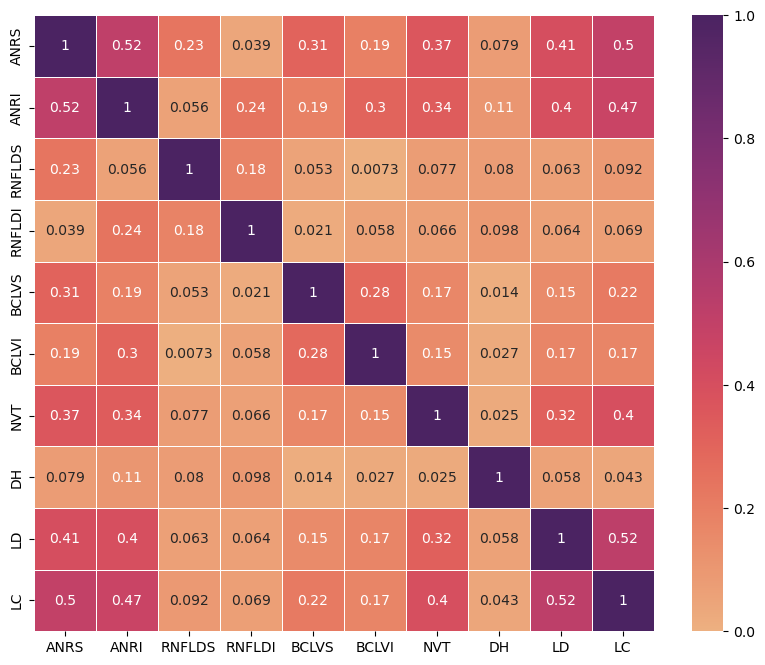
\includegraphics[width=0.7\textwidth]{images/correlation.png}
 \caption{Matriz de correlação entre anotações adicionais.}
 \label{fig:labels_correlation}
\end{figure}

\subsubsection{Imagens}
\label{sec:dataset:images}

A aquisição das imagens foi feita em vários centros de triagem com câmeras diferentes \cite{justraigs_article}.
É possível observar grande variação de brilho, contraste e nitidez nas imagens do conjunto de dados, como ilustrado na Figura~\ref{fig:images_variations_1}.

\begin{figure}
    \centering
    \begin{subfigure}[b]{0.2\textwidth}
        \centering
        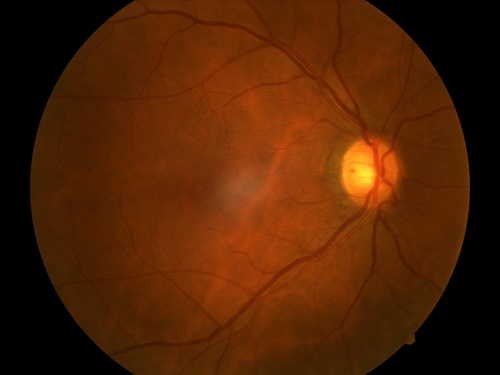
\includegraphics[width=\textwidth]{images/examples_from_dataset/TRAIN000282.JPG}
        \label{fig:images_variations_1_1}
    \end{subfigure}
    \hfill
    \begin{subfigure}[b]{0.2\textwidth}
        \centering
        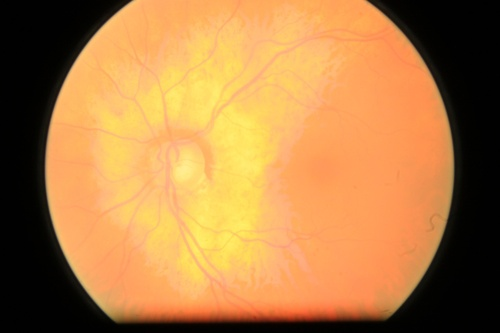
\includegraphics[width=\textwidth]{images/examples_from_dataset/TRAIN012425.JPG}
        \label{fig:images_variations_1_2}
    \end{subfigure}
    \hfill
    \begin{subfigure}[b]{0.2\textwidth}
        \centering
        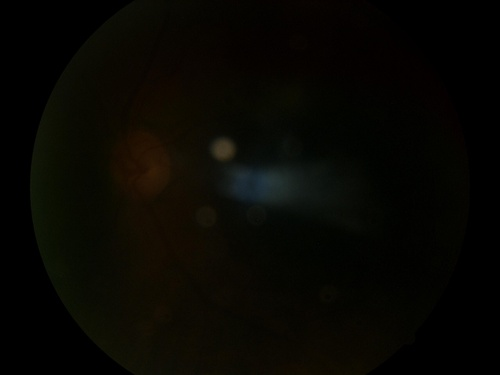
\includegraphics[width=\textwidth]{images/examples_from_dataset/TRAIN013211.JPG}
        \label{fig:images_variations_1_3}
    \end{subfigure}
    \hfill
    \begin{subfigure}[b]{0.2\textwidth}
        \centering
        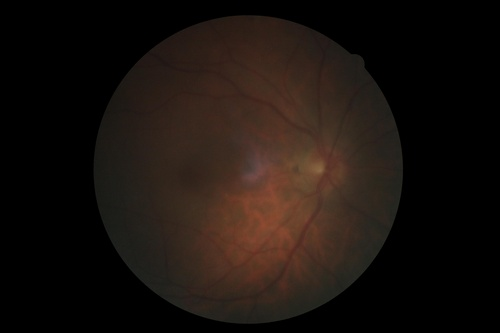
\includegraphics[width=\textwidth]{images/examples_from_dataset/TRAIN061871.JPG}
        \label{fig:images_variations_1_4}
    \end{subfigure}
    \caption{Variações de luminosidade e contraste entre imagens do JustRAIGS.}
    \label{fig:images_variations_1}
\end{figure}

Nota-se também a presença de artefatos de aquisição variados em parte das imagens, como mostrado na Figura~\ref{fig:images_variations_2}.

\begin{figure}
    \centering
    \begin{subfigure}[b]{0.2\textwidth}
        \centering
        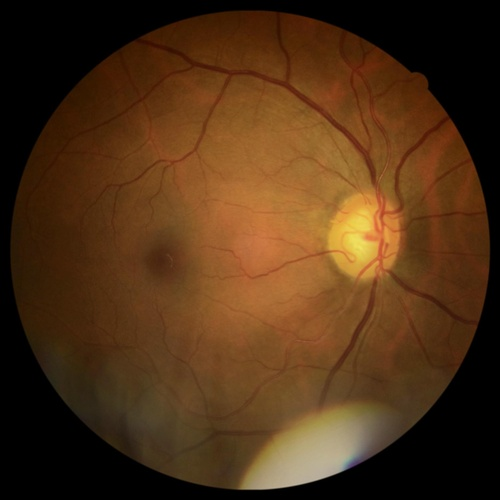
\includegraphics[width=\textwidth]{images/examples_from_dataset/TRAIN025848.JPG}
        \label{fig:images_variations_2_1}
    \end{subfigure}
    \hfill
    \begin{subfigure}[b]{0.2\textwidth}
        \centering
        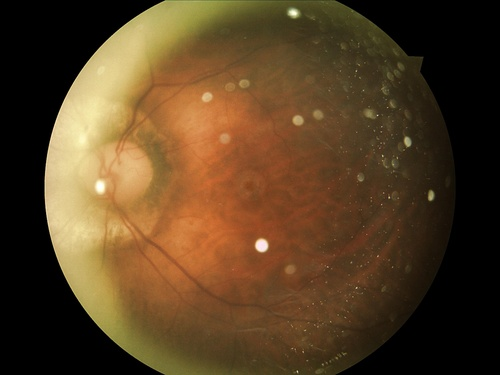
\includegraphics[width=\textwidth]{images/examples_from_dataset/TRAIN045963.JPG}
        \label{fig:images_variations_2_2}
    \end{subfigure}
    \hfill
    \begin{subfigure}[b]{0.2\textwidth}
        \centering
        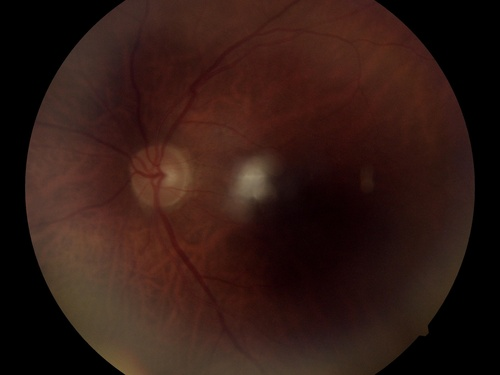
\includegraphics[width=\textwidth]{images/examples_from_dataset/TRAIN049428.JPG}
        \label{fig:images_variations_2_3}
    \end{subfigure}
    \hfill
    \begin{subfigure}[b]{0.2\textwidth}
        \centering
        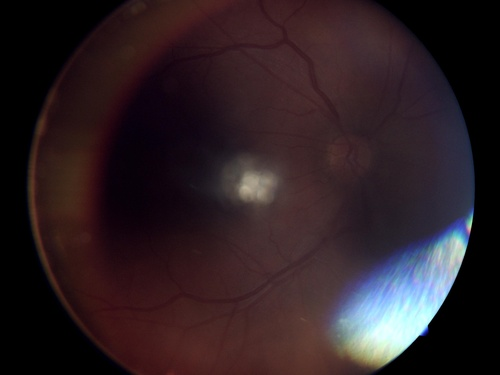
\includegraphics[width=\textwidth]{images/examples_from_dataset/TRAIN065536.JPG}
        \label{fig:images_variations_2_4}
    \end{subfigure}
    \caption{Imagens com artefatos de aquisição variados.}
    \label{fig:images_variations_2}
\end{figure}

\subsubsection{Divisão entre treino e teste}
\label{sec:dataset:split}

%% CSS: Acho que falta explicar um pouco mais, veja o que você acha de incorporar a informação abaixo no texto:
% Com 10 anotações adicionais binárias (0 ou 1), existem $2^10$ configurações possíveis. Na prática, algumas configurações são muito mais prováveis e a imensa maioria não será observada no conjunto de dados. A amostragem estratificada busca igualar a frequência de cada configuração, entre conjunto de treinamento e de teste.
%% LZT: ajustado

O conjunto de dados foi dividido na proporção 80\% para treinamento e 20\% para teste. Para realizar essa divisão, o conjunto foi inicialmente dividido entre NRG e RG. Para a porção de NRG, foi feita uma divisão aleatória simples. Já para a porção de RG, com o intuito de preservar a proporção das anotações adicionais, foi realizada uma amostragem estratificada utilizando a classe \emph{StratifiedShuffleSplit} e o método \emph{split} da biblioteca \emph{scikit-learn}.

A amostragem estratificada visa preservar, entre os conjuntos de treino e teste, a frequência relativa de cada classe. Como existem 10 anotações binárias, teoricamente seriam possíveis $2^{10}$ configurações diferentes. Na prática, no entanto, algumas combinações são muito mais frequentes, enquanto a imensa maioria sequer ocorre no conjunto de dados, de forma que não existem representantes suficientes para realizar a divisão nestes casos. Dessa forma, não foi possível estratificar diretamente considerando todas as anotações simultaneamente. Em vez disso, todas as possíveis permutações com 2, 3, 4 e 5 anotações adicionais foram testadas. O uso de mais de 6 anotações se mostrou impraticável devido à escassez de representantes.

Para escolher a melhor combinação de anotações adicionais, foi utilizada uma métrica baseada na soma dos quadrados da diferença entre a proporção obtida e a desejada para cada anotação entre os dois conjuntos. Quanto menor a pontuação, mais balanceada e representativa era a divisão. Essa abordagem garantiu que a representatividade das anotações adicionais fosse preservada entre os conjuntos, mesmo para classes com baixa ocorrência.

\subsection{Sistema proposto}
\label{sec:pipeline}

O processo de detecção automatizada de glaucoma proposto neste trabalho envolve três etapas principais: (i) a segmentação do disco óptico na imagem de fundo de olho; (ii) a classificação da imagem como caso referenciável (RG) ou não referenciável (NRG), com base na região segmentada; e (iii) a identificação das razões que justificam a referência, por meio de um classificador multi-rótulo (\emph{multi-label}), utilizando nas anotações adicionais presentes no JustRAIGS. A Figura~\ref{fig:proposed_system} mostra um diagrama do sistema.

\begin{figure}[h!]
\centering
\scalebox{0.85}{
    \begin{tikzpicture}[
        node distance=2.5cm and 1.8cm,
        every node/.style={draw, align=center, rounded corners, font=\small, minimum width=2.8cm, minimum height=1cm},
        arrow/.style={-Latex, thick}
    ]
    
    % Nodes
    \node (input) {Imagem de\\fundo de olho};
    \node (segmentador) [right=of input] {Segmentador de\\Disco Óptico};
    \node (classificador_bin) [right=of segmentador] {Classificador Binário\\(RG ou NRG)};
    \node (saida_bin) [above=of classificador_bin, draw=none] {Saída: RG ou NRG};
    \node (classificador_multi) [right=of classificador_bin] {Classificador\\Multi-rótulo\\(10 razões)};
    \node (saida_multi) [above=of classificador_multi, draw=none] {Saída: Razões};
    \node (saida_failure) [above=of segmentador, draw=none] {Saída: Falha na segmentação};
    
    % Connections 
    \draw[arrow] (input) -- (segmentador);
    \draw[arrow] (segmentador) -- (classificador_bin) node[midway, below, font=\scriptsize, draw=none, fill=none] {Disco\\encontrado};
    \draw[arrow] (segmentador.north) -- (saida_failure) node[midway, right, font=\scriptsize, draw=none, fill=none] {Falha na\\segmentação};
    \draw[arrow] (classificador_bin) -- (classificador_multi);
    \draw[arrow] (classificador_bin) -- (classificador_multi) node[midway, below, font=\scriptsize, draw=none, fill=none] {Se RG};
    \draw[arrow] (classificador_bin.north) -- (saida_bin.south);
    \draw[arrow] (classificador_multi.north) -- (saida_multi.south);
    
    \end{tikzpicture}
}
\caption{Diagrama do sistema proposto.}
\label{fig:proposed_system}
\end{figure}


\subsection{Segmentação da região de interesse}
\label{sec:segmentation}

As características visuais associadas ao glaucoma, no exame de fundo de olho, estão ou no disco óptico ou em seu entorno \cite{weinreb_2016}. Portanto, para melhor aproveitamento da rede neural classificadora, segmentamos as imagens na região do disco antes de utilizá-las em um classificador.

Para realizar essa segmentação, foi utilizado um modelo de aprendizagem profunda chamado Ultralytics YOLO11, capaz de realizar múltiplas tarefas de visão computacional em tempo real, como detecção de objetos, segmentação, classificação ou estimativa de pose humana. Ele pode ser treinado em novas bases de dados para aplicações específicas. Para cada tarefa existe uma família de modelos com quantidades de parâmetros diferentes \cite{YOLO_2023}. Escolhemos o modelo \emph{yolo11m} para detecção de objetos.

Para treinar o YOLO, foram aleatoriamente selecionadas 1400 imagens do conjunto de treinamento: 1000 para treino, 200 para validação e 200 para teste. Em cada um dos conjuntos a proporção de RG foi de 20\%. Para cada imagem, o disco óptico foi manualmente anotado por meio de uma caixa delimitadora alinhadas aos eixos definida por dois pontos. As anotações foram feitas com o software AnyLabeling \cite{anylabeling}.

\begin{figure}[htb]
 \centering
 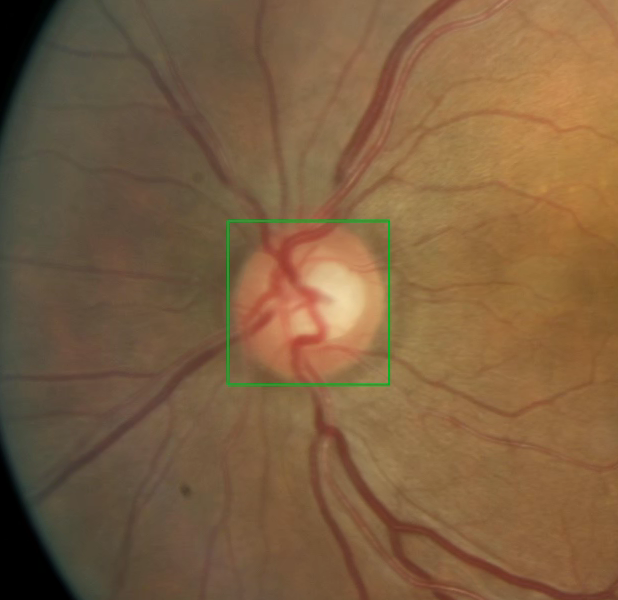
\includegraphics[width=0.3\textwidth]{images/disk_labeling.png}
 \caption{Disco óptico anotado no software AnyLabeling. Imagem original obtida do banco de dados JustRAIGS.}
 \label{fig:disk_labeling}
\end{figure}

Foi feito o treinamento do segmentador com 100 épocas utilizando os parâmetros padrões do YOLO. Após o treinamento, no conjunto de validação o modelo atingiu precisão e \emph{recall} 1, mAP50 0,995 e mAP50-95 0,945. No teste, apresentou precisão 0,995, \emph{recall} 1, mAP50 0,995 e mAP50-95 0,936.

%% LZT: para pensar... por que não usar o parâmetro 'max_det' do YOLO que limita o número de detecções máximas em uma imagem?
Em seguida, o segmentador foi aplicado para todo o conjunto de treinamento definido anteriormente na Seção~\ref{sec:dataset:split}. Das 81.138 imagens, em 80.725 (99,49\%) o modelo identificou um disco óptico, em 332 (0,41\%) mais de uma detecção foi retornada e em 81 (0,10\%) nenhuma. Para todas as detecções, utilizamos o \emph{score} mínimo de 0,25, valor padrão do YOLO.
% [LZT] TODO: rever score mínimo, talvez usar um valor mais alto. inspecionar as imagens com score mais baixo

Analisando as 332 imagens para as quais o modelo retornou mais de uma predição, identificamos alguns artefatos de aquisição predominantes que confundiram o modelo. Algumas imagens com múltiplas detecções são apresentados na Figura~\ref{fig:multiple_boxes}.

\begin{figure}
    \centering
    \begin{subfigure}[b]{0.47\textwidth}
        \centering
        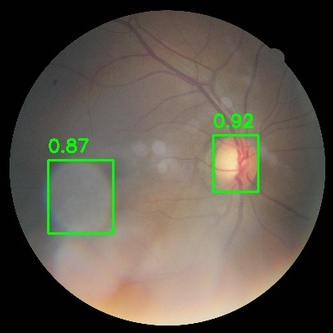
\includegraphics[width=\textwidth]{images/multiple_boxes/TRAIN003802_boxes.jpg}
        \label{fig:multiple_boxes_1}
    \end{subfigure}
    \hfill
    \begin{subfigure}[b]{0.47\textwidth}
        \centering
        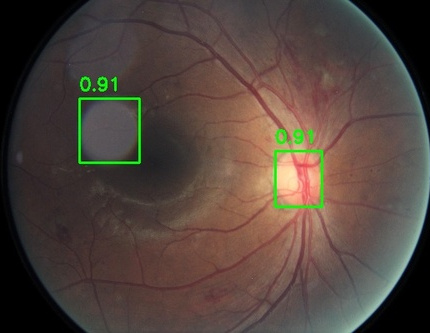
\includegraphics[width=\textwidth]{images/multiple_boxes/TRAIN031744_boxes.jpg}
        \label{fig:multiple_boxes_2}
    \end{subfigure}
    \break
    \begin{subfigure}[b]{0.47\textwidth}
        \centering
        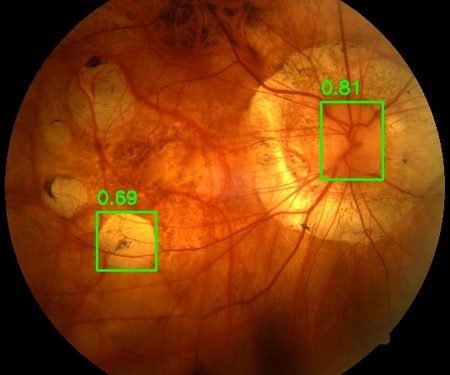
\includegraphics[width=\textwidth]{images/multiple_boxes/TRAIN011494_boxes.jpg}
        \label{fig:multiple_boxes_3}
    \end{subfigure}
    \hfill
    \begin{subfigure}[b]{0.47\textwidth}
        \centering
        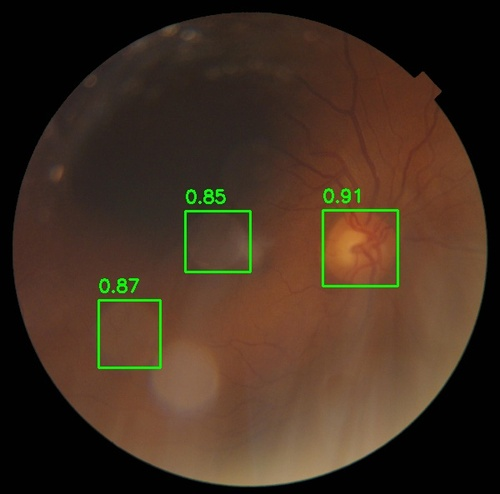
\includegraphics[width=\textwidth]{images/multiple_boxes/TRAIN031299_boxes.jpg}
        \label{fig:multiple_boxes_4}
    \end{subfigure}
    \caption{Imagens com múltiplas detecções pelo YOLO e \emph{score} atribuído.}
    \label{fig:multiple_boxes}
\end{figure}

Por outro lado, analisando as 81 imagens em que nenhuma detecção foi retornada, não conseguimos identificar uma causa predominante para a ausência de detecções. Listamos algumas das características dessas imagens, que se manifestam de formas variadas:
\begin{itemize}[noitemsep,topsep=0pt]
    \item disco óptico com limites pouco definidos;
    \item imagens com baixo contraste em que disco óptico aparece ``apagado'';
    \item imagens desfocadas ou com baixa nitidez;
    \item lesões ou deformações anatômicas diversas ao redor do disco óptico.
\end{itemize}
Alguns exemplos são apresentados na Figura~\ref{fig:images_no_box}.

\begin{figure}
    \centering
    \begin{subfigure}[b]{0.47\textwidth}
        \centering
        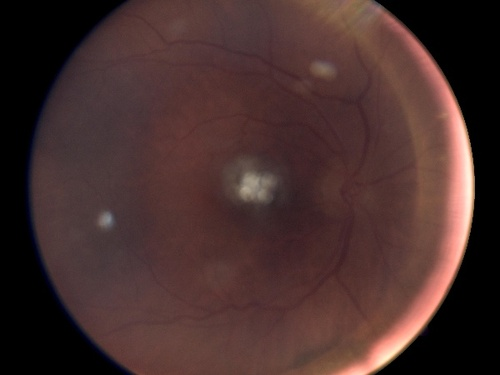
\includegraphics[width=\textwidth]{images/no_box/TRAIN000883_boxes.jpg}
        \label{fig:images_no_box_1}
    \end{subfigure}
    \hfill
    \begin{subfigure}[b]{0.47\textwidth}
        \centering
        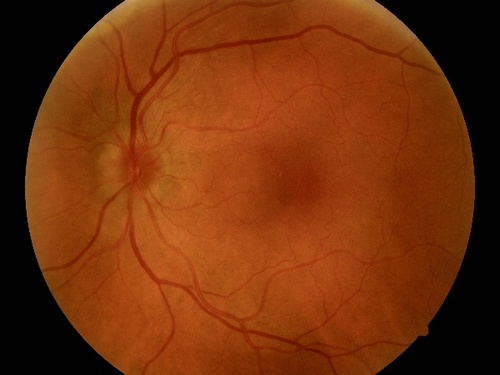
\includegraphics[width=\textwidth]{images/no_box/TRAIN045856_boxes.jpg}
        \label{fig:images_no_box_2}
    \end{subfigure}
    \break
    \begin{subfigure}[b]{0.47\textwidth}
        \centering
        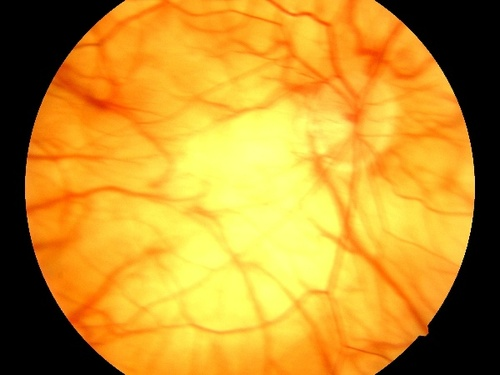
\includegraphics[width=\textwidth]{images/no_box/TRAIN046833_boxes.jpg}
        \label{fig:images_no_box_3}
    \end{subfigure}
    \hfill
    \begin{subfigure}[b]{0.47\textwidth}
        \centering
        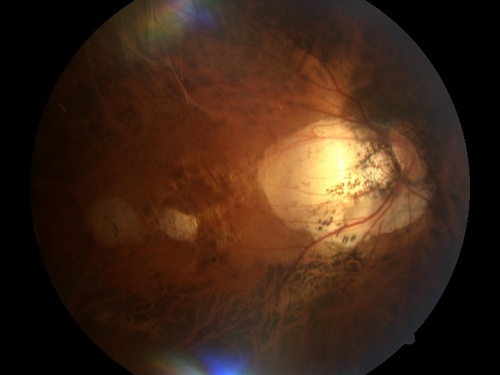
\includegraphics[width=\textwidth]{images/no_box/TRAIN099284_boxes.jpg}
        \label{fig:images_no_box_4}
    \end{subfigure}
    \caption{Imagens sem detecção pelo YOLO.}
    \label{fig:images_no_box}
\end{figure}

Resolvemos então escolher aleatoriamente 100 imagens dentre as 332 com mais de uma detecção para treinar um novo segmentador. Foram anotadas manualmente e incluídas no conjunto de dados usado anteriormente, 50, 25 e 25 imagens para treino, validação e teste, respectivamente. Devido à falta de experiência médica para identificar corretamente o disco óptico  em casos difíceis, adotamos uma postura cautelosa em não anotar as imagens para as quais o modelo não retornou nenhum resultado. Em uma aplicação real, casos como estes seriam encaminhados para avaliação de um médico. Um novo treinamento foi feito então, utilizando os mesmos parâmetros do anterior.

Desta vez, na validação o modelo atingiu precisão e \emph{recall} 1, mAP50 0,995 e mAP50-95 0,944, enquanto que no teste atingiu precisão 0,999, \emph{recall} 0,991, mAP50 0,995 e mAP50-95 0,934.

Ao aplicar esta segunda geração em todo o conjunto de treino, desta vez, o modelo identificou apenas um disco óptico em 81.016 imagens (99,85\%), devolveu mais de uma detecção em 63 (0,08\%) e nenhuma detecção em 59 (0,07\%).

% IMAGENS USADAS NO YOLO
%       gen1  new  gen2
% total 1400  100  1500
% train 1000   50  1050
% val    200   25   225
% test   200   25   225


\subsection{Classificação binária}
\label{sec:binary_classification}

Com as regiões de interesse já extraídas, a etapa de classificação binária consistiu em treinar um modelo capaz de distinguir entre casos referenciáveis para glaucoma (RG) e não referenciáveis (NRG). Para isso, utilizamos uma rede neural convolucional moderna empregando transferência de aprendizagem a partir de um modelo pré-treinado, como descrito a seguir.

Partindo de um modelo ResNet50 pré treinado no conjunto de dados ImageNet, removemos a camada superior e adicionamos uma camada GlobalAveragePooling2D, duas camadas totalmente conectadas de tamanhos 1024 e 256 com função de ativação ReLU e uma camada totalmente conectada de saída de tamanho 1 com função sigmoide, própria para classificação binária. Entre as novas camadas, foi aplicado \emph{dropout} com taxa de 50\%. Também experimentamos com uma arquitetura mais simples, de apenas uma camada totalmente conectada de tamanho 512 antes da saída, e outra arquitetura mais complexa, com camadas de tamanho na sequência 4096, 2048, 1024, 256 e saída.


As imagens disponíveis no conjunto de treino definido na Seção~\ref{sec:dataset:split} foram subdivididas entre treino e validação para a etapa de treinamento do classificador. A divisão foi realizada de forma estratificada, mantendo a proporção entre as classes, alocando 80\% das imagens para o treinamento e 20\% para a validação, conforme o processo descrito anteriormente.


%% CSS: Conferir a questão do espelhamento; mais abaixo, quando discute aumentação, o texto diz que foi aplicado flip horizontal aleatório. Está dessa maneira mesmo (o espelhamento ocorre agora E possivelmente na aumentação)?
%% LZT: sim, o espelhamento acontece nas duas etapas, dessa maneira as imagens RG vão ser vistas duas vezes, mas com aumentações diferentes
%% LZT: agora percebi que a proporção entre as classes ficou diferente no conjunto de treinamento (1:2) e no de validação (1:4). Isso é um problema? Talvez precise explicar melhor isso no texto
%% CSS, sobre o ponto acima: Isso pode ser um problema se afetar o cálculo das métricas, por exemplo, se a precisão de treinamento for diferente da precisão de validação. De resto, poderia ser entendido como uma escolha de treinamento. Nós podemos mostrar para o algoritmo algumas imagens com maior frequência, não é um erro conceitual.

Com o objetivo de contornar o desbalanceamento entre as duas classes, todas as 2.610 imagens RG disponíveis no conjunto de treinamento foram espelhadas horizontalmente e salvas como novas imagens. Além disso, apenas um subconjunto de 10 mil imagens NRG aleatoriamente selecionadas foi utilizado, resultando em uma proporção entre as duas classes de aproximadamente 1 RG para 2 NRG. Em números absolutos, foram no conjunto de treinamento 4176 (2088 x 2) imagens RG e 8000 imagens NRG, enquanto que para validação foram 522 e 2000 imagens de cada classe respectivamente. Como não aplicamos o espelhamento no conjunto de validação, a proporção foi de aproximadamente 1 RG para 4 NRG. Também experimentamos uma subamostragem de NRG mais agressiva, para que a proporção fosse de 1 para 3, mas essa configuração apresentou resultado inferior à anterior.

Antes de serem utilizadas no classificador, todas as imagens foram recortadas no entorno do disco óptico detectado pelo segmentador. A região do corte foi definida com as coordenadas devolvidas pelo modelo, acrescidas de uma margem de 50\% para cada eixo.

% IMAGENS USADAS NO CLASSIFICADOR
% NRG   10.000
% RG     5.220 (2.610 x 2)
% total 15.220

Durante o treinamento, aplicamos algumas técnicas de aumentação de dados nas imagens:

\begin{itemize}[noitemsep]
    \item \textbf{Translação}: desloca a imagem vertical e horizontalmente;
    \item \textbf{Rotação}: gira a imagem por um ângulo aleatório;
    \item \textbf{Zoom}: aproxima ou afasta a imagem;
    \item \textbf{Espelhamento horizontal}: espelha horizontalmente a imagem com 50\% de chance;
    \item \textbf{Brilho}: aumenta ou diminui o brilho;
    \item \textbf{Contraste}: ajusta aleatoriamente o contraste;
    \item \textbf{Cor}: converte a imagem de RGB para HSV, ajusta aleatoriamente o canal de cor (hue) e converte de volta para RGB.
\end{itemize}

Inicialmente experimentamos apenas com as transformações de translação, rotação, zoom e espelhamento, chamadas de transformações geométricas, que apenas movimentam a imagem. Posteriormente, experimentamos com as transformações de brilho, cor e contraste, chamadas de transformações fotométricas, que alteram o valores dos pixels. A Figura~\ref{fig:augmentations} mostra alguns exemplos de imagens antes e depois de passarem pelas transformações.

\begin{figure}[htb]
 \centering
 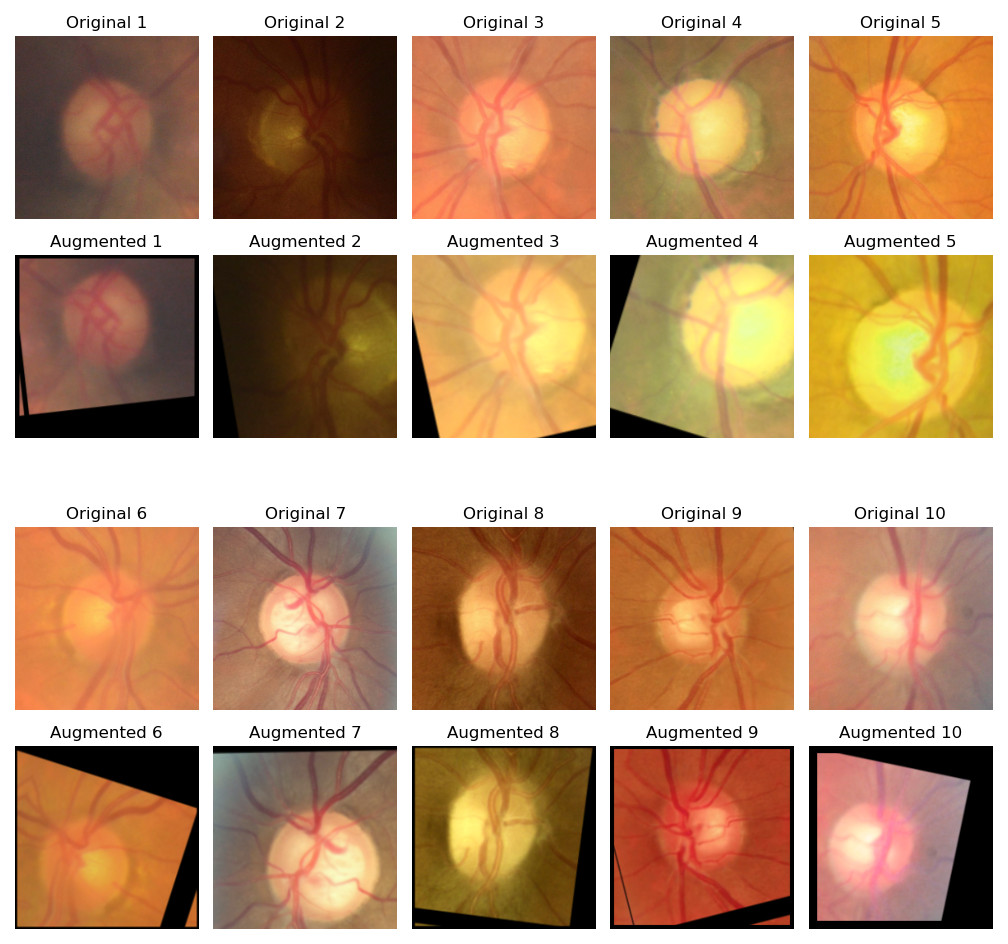
\includegraphics[width=1.0\textwidth]{images/augmentations.jpg}
 \caption{Imagens originais e após aplicação das aumentações de dados.}
 \label{fig:augmentations}
\end{figure}

Fizemos experimentos com dois processos de treinamento: em duas etapas e em etapa única. O processo de duas etapas consiste em dividir o treinamento em uma primeira fase em que os pesos do modelo original são congelados e somente os pesos da novas camadas superiores são ajustados e em uma segunda fase, conhecida como ajuste fino (\emph{fine-tuning}), em que todos os pesos são descongelados e o modelo é ajustado por inteiro a uma taxa de aprendizagem inferior. O processo de etapa única é equivalente ao ajuste fino, o treinamento já se inicia ajustando todos os pesos da rede à uma taxa de aprendizagem baixa.

As etapas de treinamento fizeram uso de parada antecipada (\emph{early stopping}), uma técnica de regularização que interrompe o treinamento ao detectar que não houve melhora no desempenho do modelo no conjunto de validação após determinada quantidade de épocas. Como métrica a ser monitorada usamos a sensibilidade em 95\% de especificidade.

Utilizamos o otimizador \emph{ADAM}, com taxa de aprendizagem de $10\textsuperscript{-4}$ na primeira etapa e $10\textsuperscript{-5}$ no ajuste fino. Nos experimentos com somente uma etapa, utilizamos a mesma taxa de aprendizagem do ajuste fino. Como função de perda utilizamos a entropia cruzada binária (\emph{binary crossentropy}).

A Tabela~\ref{tab:modelos_class_binaria} apresenta um quadro resumo das configurações de alguns dos experimentos que fizemos. O tamanho da rede se refere as camadas superiores adotadas na construção do modelo conforme descrito anteriormente, o processo se refere ao processo de treinamento em uma ou duas etapas e aumentações são as aumentações aplicadas nas imagens. Os modelos foram nomeados com base em suas configurações, utilizando as seguintes convenções: ``P'', ``M'' ou ``G'' para o tamanho da rede; ``1'' ou ``2'' para indicar a quantidade de etapas de treinamento; e o sufixo ``f'' quando há aplicação de transformação fotométrica.

%% [CSS] Sugestão: nomear os modelos pelas colunas da tabela usando {M, G, P} para o tamanho; {1,2} para processo e 'f' quando também há transformação fotométrica. Os nomes então seriam: M2, G2, M2f, M1f e P1
%% LZT: gostei das sugestões. No caso, o último não seria P1f?

\begin{table}[h]
\centering
\begin{tabular}{cccc}
\toprule
\textbf{Modelo} & \textbf{Tamanho da rede} & \textbf{Processo} & \textbf{Aumentações} \\ 
\midrule
M2  & Médio   & Duas etapas  & Geométricas \\                % 018
G2  & Grande  & Duas etapas  & Geométricas \\                % 021
M2f & Médio   & Duas etapas  & Geométricas e fotométricas \\ % 023
M1f & Médio   & Etapa única  & Geométricas e fotométricas \\ % 025
P1f & Pequeno & Etapa única  & Geométricas e fotométricas \\ % 026
\bottomrule
\end{tabular}
\caption{Resumo dos modelos treinados com diferentes processos e tipos de aumentação.}
\label{tab:modelos_class_binaria}
\end{table}

%% CSS: acrescentei o comentário sobre o JustRAIGS, veja se concorda
% LZT: boa, concordo
Para avaliar o desempenho do classificador optamos por utilizar a sensibilidade condicionada a uma especificidade mínima de 95\%, a mesma métrica usada para avaliar a classificação binária na competição JustRAIGS. Essa escolha pode ser justificada pelo  contexto clínico da aplicação: na triagem do glaucoma, queremos minimizar o número de falsos positivos, evitando sobrecarregar o sistema de saúde com encaminhamentos desnecessários. A alta especificidade garante que os pacientes encaminhados realmente apresentem sinais relevantes de glaucoma. Ao mesmo tempo, queremos maximizar a sensibilidade, isto é, a capacidade de detectar os casos verdadeiramente positivos e garantir que não estamos deixando de encaminhá-los.

% LZT: talvez faça mais sentido mover essa discussão para a seção de resultados e discussão
%% CSS: acho que pode manter este parágrafo aqui
No contexto da identificação do glaucoma, a precisão é fortemente impactada pelo grande desbalanceamento entre as classes. Por mais que tenhamos um percentual pequeno de falsos positivos em relação ao número total de casos, em números absolutos ainda vamos ter muitos casos em comparação à quantidade de verdadeiros positivos, resultando em uma precisão baixa. Portanto, apesar de reportá-la, optamos por não nos concentrar nessa métrica.

A Tabela~\ref{tab:resultados_modelos_val} apresenta os resultados obtidos pelos modelos no conjunto de validação. O modelo G2, de maior porte, teve o pior desempenho, indicando que o aumento do tamanho da rede, isoladamente, não trouxe melhorias. A adição de aumentações fotométricas (modelo M2f) resultou em pequenos ganhos. Já a adoção de treinamento em etapa única (modelos M1f e P1f) proporcionou melhorias mais expressivas, com destaque para o modelo M1f, que alcançou a melhor sensibilidade (93,87\%). A redução do tamanho da rede no modelo P1f implicou em leve queda nas métricas, mas ainda superando os primeiros modelos avaliados.

\begin{table}[h]
    \centering
    \begin{tabularx}{\textwidth}{l*{5}{>{\centering\arraybackslash}X}}
    \toprule
    \textbf{Nome} & \textbf{Sens. em 95\%} & \textbf{AUC-ROC} & \textbf{Especif.} & \textbf{Sensitiv.} & \textbf{Precisão} \\
    \midrule
    M2  & 0,9023 & 0,9764 & 0,9665 & 0,8448 & 0,8681 \\ % 018
    G2  & 0,8851 & 0,9724 & 0,9675 & 0,8084 & 0,8665 \\ % 021
    M2f & 0,9061 & 0,9746 & 0,9675 & \textbf{0,8506} & 0,8723 \\ % 023 % sens 95 deu 0.9080 offline
    M1f & \textbf{0,9387} & \textbf{0,9807} & \textbf{0,9780} & \textbf{0,8506} & \textbf{0,9098} \\ % 025
    P1f & 0,9215 & 0,9806 & 0,9745 & 0,8391 & 0,8957 \\ % 026
    \bottomrule
    \end{tabularx}
    \caption{Resultados dos modelos avaliados no conjunto de validação.}
    \label{tab:resultados_modelos_val}
\end{table}


\subsection{Classificação multi-rótulo}
\label{sec:multi_classification}

Após a classificação binária entre casos referenciáveis (RG) e não referenciáveis (NRG), foi desenvolvido um segundo classificador com o objetivo de identificar as razões que justificam a marcação de uma imagem como RG, seguindo as anotações adicionais propostas pelo conjunto de dados JustRAIGS.

Este classificador foi treinado apenas com as imagens rotuladas como RG no conjunto de treinamento. Uma mesma imagem pode estar associada à mais de uma razão, caracterizando o problema como uma tarefa de classificação multi-rótulo (\emph{multi-label classification}) com dez saídas, correspondentes aos dez possíveis rótulos adicionais anotados pelos avaliadores.

A arquitetura do classificador multi-rótulo foi construída a partir da mesma base do classificador binário, utilizando uma ResNet50 pré-treinada no ImageNet com camadas superiores substituídas por uma \emph{GlobalAveragePooling2D} e camadas totalmente conectadas de tamanhos 1024, 256 e 10, conforme descrito na Seção~\ref{sec:binary_classification}. A diferença para o classificador binário está na camada de saída que possui dez unidades, cada uma com função de ativação sigmoide, permitindo a previsão independente de cada razão.

O treinamento foi realizado em uma única etapa, com taxa de aprendizagem de $10^{-5}$ e otimizador ADAM, empregando as mesmas técnicas de aumentação de dados e estratégias de regularização aplicadas na tarefa binária, incluindo \emph{dropout} e parada antecipada (\emph{early stopping}).

Como descrito na Seção~\ref{sec:dataset}, no conjunto de dados JustRAIGS, é possível que os avaliadores, mesmo concordando em referenciar uma imagem para glaucoma, discordem nas anotações adicionais que justificam essa decisão. O JustRAIGS não implementou um mecanismo de resolução de conflitos entre avaliadores para essas anotações, disponibilizando apenas as respostas individuais. Dessa forma, propusemos uma estratégia de construção de anotações finais contínuas, conhecidas como \emph{soft-labels}, que refletem a incerteza inerente às anotações discordantes.

O processo para definição do valor final de cada anotação adicional foi estabelecido da seguinte maneira:
\begin{itemize}[noitemsep]
    \item Consideram-se A1 e A2 como os dois avaliadores iniciais, e A3 como o especialista em glaucoma acionado em caso de discordância na anotação principal.
    
    \item \textbf{Se A1 e A2 concordam na anotação principal:}\\
    Para cada anotação adicional:
    \begin{itemize}[noitemsep]
        \item Se ambos marcaram 0, o valor final atribuído é 0.
        \item Se ambos marcaram 1, o valor final atribuído é 1.
        \item Se discordam, o valor final atribuído é 0,6, refletindo a incerteza entre os avaliadores.
    \end{itemize}

    \item \textbf{Se houve discordância na anotação principal e foi necessária a avaliação de A3:}
    \begin{itemize}[noitemsep]
        \item \textbf{Caso A3 concorde em referenciar a imagem:}\\
        Para cada anotação adicional:
        \begin{itemize}[noitemsep]
            \item Se o avaliador inicial (A1 ou A2) e A3 concordam em 0, o valor final é 0.
            \item Se concordam em 1, o valor final é 1.
            \item Se apenas o avaliador inicial marcou 1, o valor final é 0,25.
            \item Se apenas A3 marcou 1, o valor final é 0,9, atribuindo maior peso à opinião do especialista.
        \end{itemize}

        \item \textbf{Caso A3 opte por não referenciar a imagem:}
        \begin{itemize}[noitemsep]
            \item Para cada anotação adicional em que um dos avaliadores iniciais marcou 1, é atribuído o valor final de 0,05, representando um indício fraco da ocorrência da característica.
        \end{itemize}
    \end{itemize}
    
    \item \textbf{Tratamento de casos de imagens marcadas como não avaliáveis (\emph{ungradable}):}\\
    Considerando que A1 marcou a imagem como \emph{ungradable}
    \begin{itemize}[noitemsep]
        \item \textbf{Se A2 e A3 concordam em RG:}
        \begin{itemize}[noitemsep]
            \item Usamos a regra já descrita anteriormente
        \end{itemize}
        
        \item \textbf{Se A2 e A3 discordam}
        \begin{itemize}[noitemsep]
            \item Se A3 marcou RG: utilizamos as anotações de A3 diretamente
            \item Se A3 marcou NRG: as anotações de A2 recebem o valor de 0,05
        \end{itemize}
    \end{itemize}
    
\end{itemize}

Essa estratégia visa refletir a incerteza das anotações entre os avaliadores e o peso maior da opinião do especialista em casos de discordância.

Para a avaliação do desempenho do classificador multi-rótulo, utilizamos uma distância de Hamming modificada. A métrica tradicional considera a quantidade de posições que são diferentes entre dois vetores. No entanto, devido a existência de discordâncias entres os avaliadores nas anotações adicionais, optamos por ignorar no cálculo os rótulos para os quais houve desacordo entre os avaliadores. Dessa forma, a distância foi calculada somente para os rótulos em que houve consenso e normalizada pela quantidade deles. 

No conjunto de validação, o modelo atingiu uma distância de Hamming média de 0,12247. Para fins de comparação, avaliamos um classificador trivial que prevê a ausência de todas as razões (todos os rótulos iguais a zero) para todas as imagens. Esse classificador \textit{baseline} obteve uma distância de Hamming média de 0,28819, demonstrando que o modelo treinado superou a estratégia básica.

\subsection{Recursos computacionais}
\label{sec:resources}

Todos os modelos foram implementados em Python com Keras utilizando o TensorFlow v2.18.0 de backend, com exceção do YOLO (Ultralytics) que utiliza o PyTorch. As versões dos pacotes eram: Python 3.10.12, Keras 3.6.0, TensorFlow 2.18.0, Ultralytics 8.3.18.
Os códigos foram executados com o sistema operacional Pop!\_OS 22.04, kernel Linux 6.9.3, contendo instalado o driver da NVIDIA 560.35.03 e as bibliotecas NVIDIA CUDA 12.6 e NVIDIA cuDNN 9.5.1.
O computador estava equipado com um processador Intel i7-10700K, 32 GB de RAM e uma GPU NVIDIA GeForce RTX 3070.

\section{Resultados}
\label{sec:results}

Esta seção apresenta os resultados obtidos pelo sistema proposto no conjunto de teste definido na Seção~\ref{sec:dataset:split}, que não foi utilizado em nenhuma etapa de desenvolvimento. Este conjunto visa avaliar a capacidade de generalização dos modelos, isto é, seu desempenho em casos nunca antes vistos.

% FASE FINAL COM CONJUNTO DE TESTE (HOLDOUT)
% SEGMENTADOR
%   Starting from 20285 images
%   Images with no box: 19 (0.09%)
%   Images with one box: 20247 (99.81%)
%   Images with more than one box: 19 (0.09%)
%
%   Threshould 0.25
%   Mean score: 0.922
%   Median score: 0.927
%   Min score: 0.264
%   Max score: 0.951

Inicialmente, o segmentador foi aplicado a todas as 20.285 imagens do conjunto de teste. Ele retornou exatamente uma detecção de disco óptico em 20.247 imagens (99,81\%), mais de uma detecção em 19 imagens (0,09\%) e nenhuma detecção em outras 19 imagens (0,09\%). A pontuação média das detecções foi de 0,922, com mediana de 0,927. Entre as imagens anotadas como glaucoma, apenas duas não tiveram detecção.
% TRAIN054105, TRAIN058447 - RG sem detecção

As imagens com exatamente uma detecção foram então avaliadas pelo classificador binário. Diferentes modelos, treinados em diversas configurações, foram testados. O modelo P1f, treinado em etapa única com todas as técnicas de aumentação e utilizando a menor arquitetura entre as avaliadas, apresentou o melhor desempenho no conjunto de teste. Este modelo havia obtido o segundo melhor desempenho na etapa de validação. No teste, atingiu sensitividade de 0,8972 em 95\% de especificidade mínima, AUC-ROC de 0,9781, especificidade de 0,9691, sensitividade de 0,8543 e precisão de 0,4789. A Tabela~\ref{tab:resultados_modelos_test} apresenta o resumo das métricas para este e outros modelos avaliados.

\begin{table}[h]
    \centering
    \caption{Resultados dos modelos avaliados no conjunto de teste.}
    \begin{tabularx}{\textwidth}{l*{5}{>{\centering\arraybackslash}X}}
    \toprule
    \textbf{Nome} & \textbf{Sens. em 95\%} & \textbf{AUC-ROC} & \textbf{Especif.} & \textbf{Sensitiv.} & \textbf{Precisão} \\
    \midrule
    M2  & 0,8773 & 0,9726 & 0,9643 & 0,8451 & 0,4408 \\ % 018
    M2f & 0,8758 & 0,9741 & 0,9611 & 0,8420 & 0,4188 \\ % 023
    M1f & 0,8819 & 0,9765 & 0,9667 & 0,8390 & 0,4558 \\ % 025
    P1f & \textbf{0,8972} & \textbf{0,9781} & \textbf{0,9691} & \textbf{0,8543} & \textbf{0,4789} \\ % 026
    \bottomrule
    \end{tabularx}
    \label{tab:resultados_modelos_test}
\end{table}

É importante observar que a precisão obtida no conjunto de teste (0,4789) é substancialmente menor do que aquela observada na validação (0,8957), o que pode causar estranheza à primeira vista. No entanto, essa diferença é explicada pela proporção entre as classes nos conjuntos: enquanto o conjunto de validação foi balanceado para conter aproximadamente 1 imagem RG a cada 4 NRG, no conjunto de teste a proporção realista é de 1 RG para 31 NRG, a mesma do JustRAIGS como um todo. Como consequência, mesmo uma pequena taxa de falsos positivos resulta em um grande número absoluto de erros em comparação à quantidade de verdadeiros positivos, o que reduz a precisão. Apesar disso, a sensitividade em 95\% de especificidade foi mantida em um patamar elevado (89,72\%), o que reforça a robustez do modelo na triagem de glaucoma mesmo sob forte desbalanceamento.

Em seguida, dentre as 20.247 imagens com detecção única, 652 possuíam anotação positiva para glaucoma. Estas foram avaliadas pelo classificador multi-rótulo, que obteve distância de Hamming de 0,12960, valor ligeiramente superior ao obtido na validação (0,12247), mas consideravelmente inferior ao \emph{baseline} (0,28819) obtido por um classificador ingênuo.

Os resultados obtidos evidenciam a capacidade do sistema proposto em realizar a triagem de glaucoma e justificar suas decisões de forma interpretável. A Tabela~\ref{tab:final_work_comparative} apresenta uma comparação entre os resultados deste trabalho e aqueles reportados por outros estudos com o conjunto de dados JustRAIGS, conforme discutido na Seção~\ref{sec:review:related:justraigs}.

\begin{table}[h]
    \centering
    \small
    \renewcommand{\arraystretch}{1.5}
    \begin{tabularx}{\textwidth}{p{2cm}XXp{1.9cm}p{1.9cm}}
    \toprule
    \textbf{Autor(es)} & \textbf{Arquitetura(s)} & \textbf{Estratégia adicional} & \textbf{Sensitiv. 95\% Esp.} & \textbf{Dist. de Hamming} \\
    \midrule
    Galdran e Ballester \cite{justraigs_galdran} & ResNet50 & Suavização de rótulos & 94,33\%* & 0,1440* \\

    Zhang et al. \cite{justraigs_zhang} & Ensemble ResNet50 + Transformers & - & 87,00\% & 0,239 \\

    Kubrak \cite{justraigs_kubrak} & YOLOv8 + Vision Transformer & Segmentação do disco & 90,90\% & 0,1280 \\

    Lin et al. \cite{justraigs_hu_lin} & YOLOv8 + Vision Transformer & Segmentação do disco & 85,70\% & 0,1250 \\
    Presente trabalho & YOLOv8 + ResNet50 & Segmentação do disco + Suavização de rótulos & 89,72\%** & 0,1296** \\
    \bottomrule
    \end{tabularx}
    \renewcommand{\arraystretch}{1}
    \newline
    \raggedright
    \scriptsize
    \textit{Nota: os valores foram obtidos em conjuntos de teste distintos e, portanto, não são diretamente comparáveis.} \\
    (*) Métricas obtidas em subconjuntos de validação. \\
    (**) Métricas obtidas em subconjunto de teste independente. \\
    Demais valores foram reportados no conjunto de teste da competição na etapa de validação.
    \caption{Comparativo do presente trabalho com outros que utilizaram o JustRAIGS.}
    \label{tab:final_work_comparative}
\end{table}


\section{Conclusões e Trabalhos Futuros}
\label{sec:conclusions}

Este trabalho propôs o desenvolvimento de um sistema baseado em aprendizagem profunda para a detecção automatizada de casos de glaucoma em imagens de fundo de olho, utilizando a segmentação do disco óptico, a classificação binária e a identificação multi-rótulo das características clínicas justificadoras. Foram empregados redes neurais convolucionais modernas, técnicas de aumento de dados e estratégias de regularização no treinamento dos modelos.

No conjunto de teste definido, o sistema atingiu uma sensitividade de 89,72\% em 95\% de especificidade mínima e uma AUC-ROC de 0,9781 na tarefa de classificação binária. Para a tarefa de classificação multi-rótulo, obteve distância de Hamming de 0,12960, superando significativamente o \emph{baseline} de 0,28819 correspondente a um classificador ingênuo.

Comparando com trabalhos relacionados desenvolvidos com o mesmo conjunto de dados JustRAIGS, o desempenho do sistema posiciona-se de maneira competitiva.  
Na tarefa de classificação binária, Kubrak \cite{justraigs_kubrak} atingiu sensitividade de 90,90\% em 95\% de especificidade no conjunto de testes da competição, enquanto Lin et al. \cite{justraigs_hu_lin} obtiveram 85,70\%. Nosso sistema obteve 89,72\% no conjunto de teste interno.
Na tarefa multi-rótulo, Kubrak reportou distância de Hamming de 0,1280, Lin et al. \cite{justraigs_hu_lin} reportaram 0,1250, enquanto Zhang et al. \cite{justraigs_zhang} reportaram 0,239. O sistema proposto apresentou desempenho próximo desses trabalhos, com distância de Hamming de 0,12960, utilizando uma arquitetura mais simples e sem a aplicação de \emph{ensembles} ou \emph{transformers}.

Cabe ressaltar que os resultados apresentados não são diretamente comparáveis, uma vez que foram avaliados em conjuntos de teste distintos. Apesar disso, o uso de um conjunto de teste separado e não utilizado durante o treinamento permite uma comparação aproximada, fornecendo uma referência válida sobre o posicionamento do sistema proposto frente aos métodos existentes.

Desta maneira, evidenciamos que os objetivos propostos foram atingidos:
\begin{itemize}[noitemsep]
    \item Desenvolvemos um método de segmentação do disco óptico com taxa de sucesso de 99,81\%;
    \item Apresentamos um classificador binário que atingiu desempenho robusto para a triagem de glaucoma;
    \item Apresentamos um classificador multi-rótulo que atingiu desempenho comparável com os disponíveis na literatura no apontamento das razões clínicas que justificam a decisão.
    %\item Avaliamos o desempenho em cada tarefa com métricas relevantes;
    %\item Comparamos os resultados obtidos com trabalhos recentes da literatura.
\end{itemize}

% LZT para CSS: o que mais podemos colocar?
%% CSS: pode dizer que o estudo usou a distância de Hamming para avaliação multi rótulo para ficar compatível com a competição, porém não está claro que essa métrica é a mais adequada. Podem existir outras métricas que se correlacionam melhor com práticas de triagem de casos.
% LZT: adicionado

Entre as limitações do trabalho, destacamos a avaliação do classificador multi-rótulo. Foi utilizada a distância de Hamming com o objetivo de tornar a avaliação compatível com a proposta da competição, porém não está claro se esta é a métrica mais adequada para o contexto clínico. Possivelmente, outras métricas poderiam refletir melhor o desempenho em cenários de triagem. Destacamos também que o sistema foi avaliado apenas em um único conjunto de dados, sem validação externa em outras bases ou contextos clínicos.

% LZT: acha que vale incluir essa ultima afirmação?
% ..., uma limitação comum no uso de aprendizagem profunda em imagens de fundo de olho, conforme destacado por Li et al.~\cite{li_review_2021}.

% explorar o threshold do YOLO ou outros segmentadores


Como trabalhos futuros, propõe-se:
\begin{itemize}[noitemsep]
%    \item Investigar arquiteturas de última geração, como Vision Transformers (ViT), para segmentação e classificação;
    \item Explorar métodos de interpretabilidade visual para explicar as decisões do modelo;
    \item Realizar testes em bases de dados adicionais e avaliações clínicas no mundo real.
\end{itemize}

Os resultados obtidos indicam que sistemas baseados em aprendizagem profunda apresentam grande potencial como ferramenta de apoio à triagem de glaucoma, contribuindo para o diagnóstico precoce e a redução da cegueira potencialmente evitável.

% discussão legal do kubrak
% During the creation of the JustRAIGS dataset, Lemij et al. (2023) re-
% quired graders to pass the European Optic Disc Assessment Trial (EODAT)
% with an overall accuracy of at least 85% and specificity of 92% or above.
% Out of 90 experienced ophthalmologists and optometrists, only 30 passed
% this threshold (Lemij et al., 2023). Given that our pipeline achieved an
% accuracy of 94.49% and 95% specificity, it would likely also pass the EO-
% 5 discussion and conclusion 17
% DAT test. However, the third graders responsible for resolving conflicts in
% labeling needed to have a minimum accuracy of 95% (Lemij et al., 2023).
% Our architecture performed slightly below this threshold, therefore not
% outperforming the best clinicians


% [LZT] aprendizados pessoais:
% - sempre usar uma seed em operações que usam RNG
% - definir bem quais metricas serão avaliadas, e qual será a principal, antes de iniciar os experientos
% - fazer experimentos incrementais e que mudem apenas uma caracteristica para responder uma única pergunta




\newpage

%% LZT: Como fazer para não incluir a lista completa de nomes? [SBB+21] ficou muito grande
%% CSS: Parte da mudança para biblatex; suspendendo por enquanto,
% ver comentário no preâmbulo (5/9/2024)
% \printbibliography

% teste
% \bibliographystyle{alpha}%{hapalike}
% \bibliography{ref.bib}

\bibliographystyle{plain}
\bibliography{ref}


\end{document}
